\documentclass[11pt,a4paper]{article}
\usepackage[margin=2.2cm]{geometry}
\usepackage{graphicx}
\usepackage{float}
\usepackage{booktabs}
\usepackage{longtable}
\usepackage{array}
\usepackage{multirow}
\usepackage{tabularx}
\usepackage{enumitem}
\usepackage{amsmath}
\usepackage{amssymb}
\usepackage{xcolor}
\usepackage{hyperref}
\usepackage{caption}
\usepackage{subcaption}
\usepackage{tikz}
\usepackage{listings}
\usepackage{fancyhdr}
\usetikzlibrary{arrows.meta, positioning, shapes.geometric, calc}

\hypersetup{
  colorlinks=true,
  linkcolor=blue!55!black,
  urlcolor=blue!55!black,
  citecolor=blue!55!black
}

\pagestyle{fancy}
\setlength{\headheight}{15pt}
\fancyhf{}
\lhead{Reverse Modeling of Google Play Age Rating}
\rhead{Social Privacy Networks Project}
\cfoot{\thepage/\pageref{LastPage}}

\lstdefinestyle{code}{
  basicstyle=\ttfamily\small,
  breaklines=true,
  columns=fullflexible,
  frame=single,
  rulecolor=\color{black!20},
  backgroundcolor=\color{black!3},
  showstringspaces=false,
  tabsize=2
}
\lstset{style=code}

\newcommand{\code}[1]{\texttt{\footnotesize\detokenize{#1}}}
\newcommand{\projecttitle}{Black-Box Reverse Modeling and Prediction of Google Play Age Rating Questionnaire}
\newcommand{\repo}{CYH0415/OSN-Lab-Main}

\begin{document}

\begin{titlepage}
\centering
\vspace*{1.0cm}

\includegraphics[width=0.78\textwidth]{figures/head.png}

\vspace{1.8cm}

\includegraphics[width=0.24\textwidth]{figures/badge.png}

\vspace{1.6cm}
{\Large\bfseries Course Project Report on Social Privacy Networks\par}
\vspace{0.7cm}
{\Large\bfseries \projecttitle\par}

\vfill
\begin{center}
\large
\renewcommand{\arraystretch}{1.6}
\begin{tabular}{rl}
Group Members: & Bofan Chen, Yuhan Chen, Zihan Chen, Jiashun Shi, Zixuan Wang \\
Project Repository: & \url{https://github.com/CYH0415/OSN-Lab-Main} \\
Experimental Subject: & Google Play / IARC Content Rating Questionnaire \\
Prediction Target: & North American ESRB Age Rating \code{rating__north_america} \\
Core Methodology: & Automated Sampling, Data Cleaning, Feature Engineering, \\
                  & Multi-Class Machine Learning, Model Interpretability Analysis \\
\end{tabular}
\end{center}

\vspace{1.2cm}
{\large\today\par}
\end{titlepage}

\clearpage
\tableofcontents
\clearpage

\section{Abstract}

The age rating mechanism on Google Play helps parents and general users determine if an application is appropriate for minors. When developers fill out the IARC content rating questionnaire in the Google Play Developer Console, the system generates age ratings, content descriptors, and interactive elements for various territories. However, Google does not publish the exact decision rules mapping questionnaire answers to final ratings. Developers and users can only observe the inputs (questionnaire answers) and outputs (rating results) without direct access to how each question, branch, and risk factor influences the final rating. Therefore, this project treats the Google Play age rating questionnaire as a black-box system and employs automated sampling and machine learning to reverse model the mapping from questionnaire answers to the final age ratings.

In line with the course requirements, this project has successfully implemented tree-structured questionnaire inspection, automated sample submission, data cleaning and validation, feature engineering, multi-model training, model performance comparison, and rating mechanism analysis. The final dataset contains 1,265 valid samples covering three primary application categories: "All Other App Types", "Game", and "Social or Communication". The cleaned data is deterministically split into 1,012 training samples and 253 testing samples. The feature engineering stage encodes 165 raw input fields into 758-dimensional features. Specifically, 133 radio/categorical fields are one-hot encoded, and 32 checkbox fields are multi-hot encoded. Structural missingness indicators such as \code{__INACTIVE__}, \code{__NOT_APPLICABLE__}, and \code{__NONE__} are explicitly retained.

In the model training phase, we trained and compared four types of models: L1-regularized Logistic Regression, Random Forest, LightGBM, and XGBoost. Experimental results show that L1-regularized Logistic Regression achieves the best performance on the test set, with an Accuracy of 0.921, a Macro F1-score of 0.918, and a Macro One-vs-Rest AUC of 0.977. XGBoost ranks second with 0.814 Accuracy and approximately 0.810 Macro F1. After parameter tuning, Random Forest reaches 0.783 Accuracy and 0.797 Macro F1. LightGBM exhibits relatively weaker performance under this sample size and high-dimensional sparse feature setting, yielding an Accuracy of 0.680. Further analysis reveals that Google Play age ratings are primarily driven by high-risk content such as violence/gore severity, sexual content/nudity, drug references, and gambling/cash rewards. Furthermore, the tree structure of the questionnaire itself carries critical information, as the activation of certain sub-questions implicitly reflects the underlying risk path.

This report documents the experimental background, project completion status, system architecture, data collection strategy, data quality control, feature engineering, model training and tuning, results comparison, encountered challenges and solutions, group member division of labor, and directions for future improvement.

\section{Course Requirements and Project Completion}

\subsection{Understanding Project Tasks}

According to the course project guidelines, this project reverse models the Google Play age rating questionnaire as a black box. The core requirements consist of four parts:
\begin{enumerate}[leftmargin=2em]
  \item \textbf{Data Collection Strategy \& Execution}: Design a systematic and efficient sampling strategy for the tree-structured content rating questionnaire, automatically submit questionnaires and collect rating results using scripts, and acquire at least 1,000 valid and diverse samples.
  \item \textbf{Model Training \& Prediction}: Perform feature engineering on the collected questionnaire data, train multi-class age rating prediction models, compare at least three different model types, and optimize their performance.
  \item \textbf{Results Analysis}: Analyze overall model performance, investigate prediction differences among age rating classes, and explore the hidden rules within the Google Play rating mechanism (e.g., finding the most influential questions or content risk factors).
  \item \textbf{Comprehensive Report}: Compile a complete report covering the data collection strategy, dataset analysis, model training, performance evaluation, challenges and solutions, key findings, core code snippets, and crucial charts.
\end{enumerate}

The implementation goes beyond simple modeling on a static dataset, establishing a reproducible data closed-loop starting from automated web page inspection. The overall workflow is illustrated in Figure~\ref{fig:workflow}.

\begin{figure}[H]
\centering
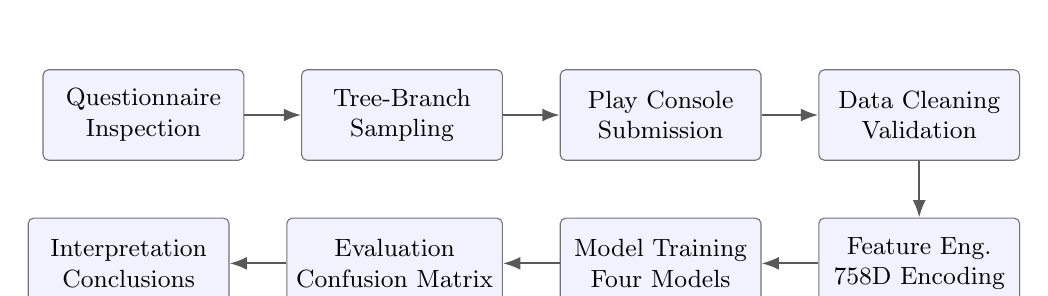
\begin{tikzpicture}[
  node distance=0.72cm,
  flowstep/.style={rectangle, rounded corners=2pt, draw=black!55, fill=blue!5, minimum width=2.55cm, minimum height=1.15cm, align=center, font=\small},
  arrow/.style={-{Latex[length=2.2mm]}, thick, draw=black!65}
]
\node[flowstep] (a) {Questionnaire\\Inspection};
\node[flowstep, right=of a] (b) {Tree-Branch\\Sampling};
\node[flowstep, right=of b] (c) {Play Console\\Submission};
\node[flowstep, right=of c] (d) {Data Cleaning\\Validation};
\node[flowstep, below=of d] (e) {Feature Eng.\\758D Encoding};
\node[flowstep, left=of e] (f) {Model Training\\Four Models};
\node[flowstep, left=of f] (g) {Evaluation\\Confusion Matrix};
\node[flowstep, left=of g] (h) {Interpretation\\Conclusions};
\draw[arrow] (a) -- (b);
\draw[arrow] (b) -- (c);
\draw[arrow] (c) -- (d);
\draw[arrow] (d) -- (e);
\draw[arrow] (e) -- (f);
\draw[arrow] (f) -- (g);
\draw[arrow] (g) -- (h);
\end{tikzpicture}
\caption{End-to-end experiment workflow. The project forms a closed loop starting from dynamic questionnaire inspection, through sampling, collection, cleaning, encoding, modeling, and interpretability analysis.}
\label{fig:workflow}
\end{figure}

\subsection{Project Completion Status}

\begin{table}[H]
\centering
\caption{Comparison of Course Requirements and Project Completion}
\label{tab:requirements}
\renewcommand{\arraystretch}{1.35}
\begin{tabularx}{\textwidth}{p{3.8cm} X p{2.0cm}}
\toprule
Requirement & Project Completion Status & Status \\
\midrule
Tree Questionnaire Understanding & Used Playwright and Chrome CDP to inspect questions, options, parent-child dependencies, and branches for the three main categories. Generated structured outputs such as \code{question_graph.json}, \code{question_graph.md}, and \code{question_graph.html}. & Completed \\
Automated Data Collection & Wrote scripts including \code{inspect_questionnaire.mjs}, \code{run_rating_samples.mjs}, and \code{autonomous_rating_sampler.mjs} to reuse a real Chrome session for automatic questionnaire filling, submission, parsing, and result saving. & Completed \\
$\ge$ 1,000 Valid Samples & The cleaned dataset contains 1,265 valid samples (satisfying the 1,000 requirement). We also recorded 770 execution failures, 30 upstream quarantined samples, and 13 rating conflicts for audit purposes. & Completed \\
Feature Engineering & Excluded all rating labels except the target column to prevent data leakage. Kept only \code{category} and \code{answer__*} to construct a 758-dimensional feature space from 165 raw inputs. & Completed \\
$\ge$ 3 Prediction Models & Trained and compared four models: Logistic Regression, Random Forest, LightGBM, and XGBoost. & Completed \\
Tuning & Optimized hyperparameters and applied regularizations for all models. Compared Accuracy, Macro F1, Weighted F1, and Macro AUC. & Completed \\
Results Analysis & Analyzed overall accuracy, category-level differences, confusion matrices, feature importance, structural missingness, and model redundancy. & Completed \\
Comprehensive Report & Compiled this complete report using LaTeX, incorporating core code, statistics, and figures. & Completed \\
\bottomrule
\end{tabularx}
\end{table}

\section{Experimental Background and Problem Definition}

\subsection{Google Play Age Rating Mechanism}

Applications published on Google Play are required to complete a content rating questionnaire provided by the IARC system. Developers must answer whether the application contains violence, gore, horror, sexual content, drugs, gambling, user interaction, location sharing, or digital purchases. Based on these answers, the system generates ratings for different jurisdictions (e.g., North American ESRB, European PEGI, German USK, Australian ACB, etc.).

This project selects the North American ESRB rating as the primary prediction target, namely \code{rating__north_america}. This label contains five categories, as listed in Table~\ref{tab:labels}.

\begin{table}[H]
\centering
\caption{North American ESRB Age Rating Labels}
\label{tab:labels}
\renewcommand{\arraystretch}{1.25}
\begin{tabular}{cll}
\toprule
Index & Label & Meaning \\
\midrule
0 & Everyone & Suitable for all ages \\
1 & Everyone 10+ & Suitable for ages 10 and older \\
2 & Teen & Suitable for teens \\
3 & Mature 17+ & Suitable for ages 17 and older \\
4 & Adults only 18+ & Explicitly for adults aged 18 and older \\
\bottomrule
\end{tabular}
\end{table}

\subsection{Black-Box Reverse Modeling Goal}

From a machine learning perspective, the Google Play age rating questionnaire can be abstracted as an unknown function:
\[
f: X \rightarrow Y,
\]
where $X$ represents the questionnaire answer state and $Y$ represents the final age rating label. Since the rules of $f$ are hidden by Google, we query the system to collect input-output samples:
\[
\mathcal{D} = \{(x_i, y_i)\}_{i=1}^{n}.
\]
The goal of the project is to learn an approximation function $\hat{f}$ that can predict the ESRB rating given new questionnaire answers:
\[
\hat{y} = \hat{f}(x).
\]

Compared to standard tabular classification tasks, this task presents several unique challenges:
\begin{enumerate}[leftmargin=2em]
  \item \textbf{Dynamic Tree Structure}: Different application categories trigger different sets of questions. Within a category, selecting a specific option determines whether subsequent sub-questions appear.
  \item \textbf{Non-Random Missingness}: Untriggered sub-questions are not missing due to data corruption, but represent structural states dictated by questionnaire logic.
  \item \textbf{Massive Sample Space}: Combinatorial explosion prevents exhaustive search of all radio and checkbox options, making manual sampling infeasible.
  \item \textbf{Imbalanced Classes}: Intermediate categories (e.g., Everyone 10+) have fewer samples, and boundaries (e.g., Teen vs. Mature 17+) are highly ambiguous.
  \item \textbf{Web Automation Hurdles}: Google Play Console page interactions involve login sessions, draft saving, loading delays, overlays, and asynchronous updates.
\end{enumerate}

\section{System Architecture and Repository Structure}

\subsection{Code Repository Structure}

The code repository is organized into modular directories corresponding to web automation, data collection, cleaning, feature engineering, and model training. The main modules are summarized in Table~\ref{tab:repo}.

\begin{longtable}{p{6.2cm}p{8.4cm}}
\caption{Key Modules in the Project Repository}
\label{tab:repo}\\
\toprule
Path & Purpose \\
\midrule
\endfirsthead
\toprule
Path & Purpose \\
\midrule
\endhead
\code{scripts/}\\\code{inspect_questionnaire.mjs} & Uses Playwright and Chrome CDP to inspect the dynamic question structures, options, and parent-child dependencies of the Google Play IARC questionnaire. \\
\code{scripts/run_rating_samples.mjs} & Connects to debug Chrome, fills out the questionnaire using specified samples, saves the draft, parses final ratings, and records results/failures. \\
\code{scripts/}\\\code{autonomous_rating_sampler.mjs} & Fully automated loop for candidate generation, batch selection, filling, parsing, and retrying to achieve the target 1,000 valid samples. \\
\code{data_categories/} & Contains inspected question graphs, questionnaire trees, interactive HTML visualizers, and risk annotations for the three categories. \\
\code{rating_artifacts/} & Stores raw collected samples, execution logs, failure events, evidence screenshots, and batch summaries. \\
\code{dataset_v2/} & Retains semantically deduplicated datasets, debug evidence, execution errors, quarantined samples, rating conflicts, and schemas. \\
\code{task3_data_cleaning/} & Python cleaning scripts, outputting \code{clean_dataset.csv}, \code{train.csv}, \code{test.csv}, the data dictionary, and cleaning reports. \\
\code{task4_feature_engineering/} & Scripts and features for encoding categorical/checkbox inputs into sparse matrices, outputting feature dictionaries, label mappings, and class weights. \\
\code{task5_1_lightgbm\&xgboost/} & Notebooks for training, tuning, evaluating, and plotting confusion matrices for LightGBM and XGBoost models. \\
\code{task5_2_logistic_regression}\\\code{\&random_forest/} & Scripts, models, classification reports, metrics, and confusion matrices for Logistic Regression and Random Forest. \\
\bottomrule
\end{longtable}

\subsection{Technology Stack}

The project is implemented using Node.js and Python. The web automation components rely on Playwright and the Chrome DevTools Protocol. Data cleaning and model training are powered by pandas, scikit-learn, scipy sparse, joblib, LightGBM, and XGBoost.

\begin{table}[H]
\centering
\caption{Project Technology Stack}
\label{tab:tech}
\renewcommand{\arraystretch}{1.25}
\begin{tabularx}{\textwidth}{p{3.5cm}X}
\toprule
Module & Technologies and Tools \\
\midrule
Web Automation & Playwright, Chrome CDP, Dedicated Chrome Profile, Google Play Developer Console \\
Data Formats & JSONL, CSV, Schema JSON, Run Configs, Debug Evidence \\
Data Processing & Python, pandas, scipy sparse, deterministic hashing \\
Modeling & scikit-learn Logistic Regression, Random Forest, LightGBM, XGBoost \\
Evaluation & Accuracy, Macro F1, Weighted F1, Macro OvR AUC, classification reports, confusion matrices \\
Reporting & LaTeX, TikZ, booktabs, longtable \\
\bottomrule
\end{tabularx}
\end{table}

\section{Questionnaire Structure Inspection and Sampling Design}

\subsection{Questionnaire Structure Inspection}

The Google Play content rating questionnaire is not a static form, but a dynamic, tree-structured questionnaire. The project must first identify the questions, options, parent-child dependencies, and reachable paths for each application category. The usage of the inspection script is detailed in \code{docs/questionnaire-inspection.md}. Since Google blocks default Playwright headless login, we use a real Chrome instance connected via CDP:

\begin{lstlisting}[language=bash, caption={Typical command for questionnaire structure inspection}]
# Start real Chrome with remote debugging and log into developer account
bash scripts/open_debug_chrome.sh

# Reuse the Chrome session to inspect the questionnaire structure
CDP_URL="http://127.0.0.1:9222" npm run inspect:questionnaire
\end{lstlisting}

The inspection script generates three core files:
\begin{enumerate}[leftmargin=2em]
  \item \code{question_graph.json}: Compact question graph where each question lists its options, and each option lists its direct child questions.
  \item \code{questionnaire_tree.json}: Raw debug tree recording probe edges, state changes, and skipped probes.
  \item \code{question_graph.html}: Interactive local HTML visualization for manual inspection.
\end{enumerate}

\subsubsection{Google Questionnaire Structural Features}

The Google Play IARC questionnaire exhibits the following structural characteristics:
\begin{enumerate}[leftmargin=2em]
  \item \textbf{Dynamic Tree-Structured Branch Dependencies}: The questionnaire is a nested hierarchical tree rather than a flat form. A user's answer to a parent question (e.g., "Does the app contain violent content?") dynamically triggers or hides subsequent sub-questions. This parent-child dependency leads to distinct sets of reachable questions depending on the answers selected.
  \item \textbf{Diverse Interaction Controls and State Constraints}: The form primarily consists of Radio Buttons and Checkboxes. Once a Radio Button is selected, it cannot be directly deselected to return to an empty state; it can only be changed by selecting another option in the same group. Checkboxes can be toggled freely between true and false.
  \item \textbf{Stable Question and Option Identifiers}: To build an accurate graph representation, the script generates a unique, stable hash Key for each question based on its question type, prompt text, and set of available options, rather than relying on volatile DOM hierarchies or dynamic IDs. This ensures that a question's ID remains identical across different branches.
\end{enumerate}

\subsubsection{DFS Structure Inspection Algorithm}

To automatically reconstruct the questionnaire's dynamic topology, we implemented a depth-first search (DFS) inspection script in \code{scripts/inspect_questionnaire.mjs}. The core execution process is as follows:
\begin{enumerate}[leftmargin=2em]
  \item \textbf{Frontier-Based Visibility Detection}: Starting from the category selection screen, the script enters the questionnaire. It only probes questions that are currently visible on the page and lie within the current DFS search frontier, preventing invalid interactions.
  \item \textbf{Option-Triggered Observation}: For each focused question, the script clicks its options one by one. After each click, it pauses for a rendering buffer (\code{PAUSE_MS}) and observes the newly appeared or disappeared sub-questions. If clicking an option displays new questions, they are added as children of that specific option in \code{question_graph.json}.
  \item \textbf{State Recovery and Backtracking}: When a branch is fully explored and backtracking is required, the script restores the questionnaire state. Checkboxes are simply unchecked. For radio buttons, which cannot be deselected, the script either performs local restoration using recorded states or, if necessary, discards the draft, returns to the category selection page, and replays the path from the root to ensure state consistency.
  \item \textbf{Graph Output and Visualization}: After traversal, the script clean and normalizes the data into \code{question_graph.json} and the detailed trace file \code{questionnaire_tree.json}.
\end{enumerate}

Using this inspection tool, we exported the questionnaire topology for the supported categories. Figure~\ref{fig:questionnaire-structures} shows the structures of the Game and All Other App Types categories. The All Other App Types category consists of 115 questions with a wider and flatter branch structure, whereas the Game category has 91 questions with deeper, highly specialized sub-branches (e.g., gambling simulations, virtual currencies). Figure~\ref{fig:question-example} shows a localized four-level question branch exemplifying sub-question triggers.

\begin{figure}[H]
\centering
\begin{subfigure}{0.48\textwidth}
  \centering
  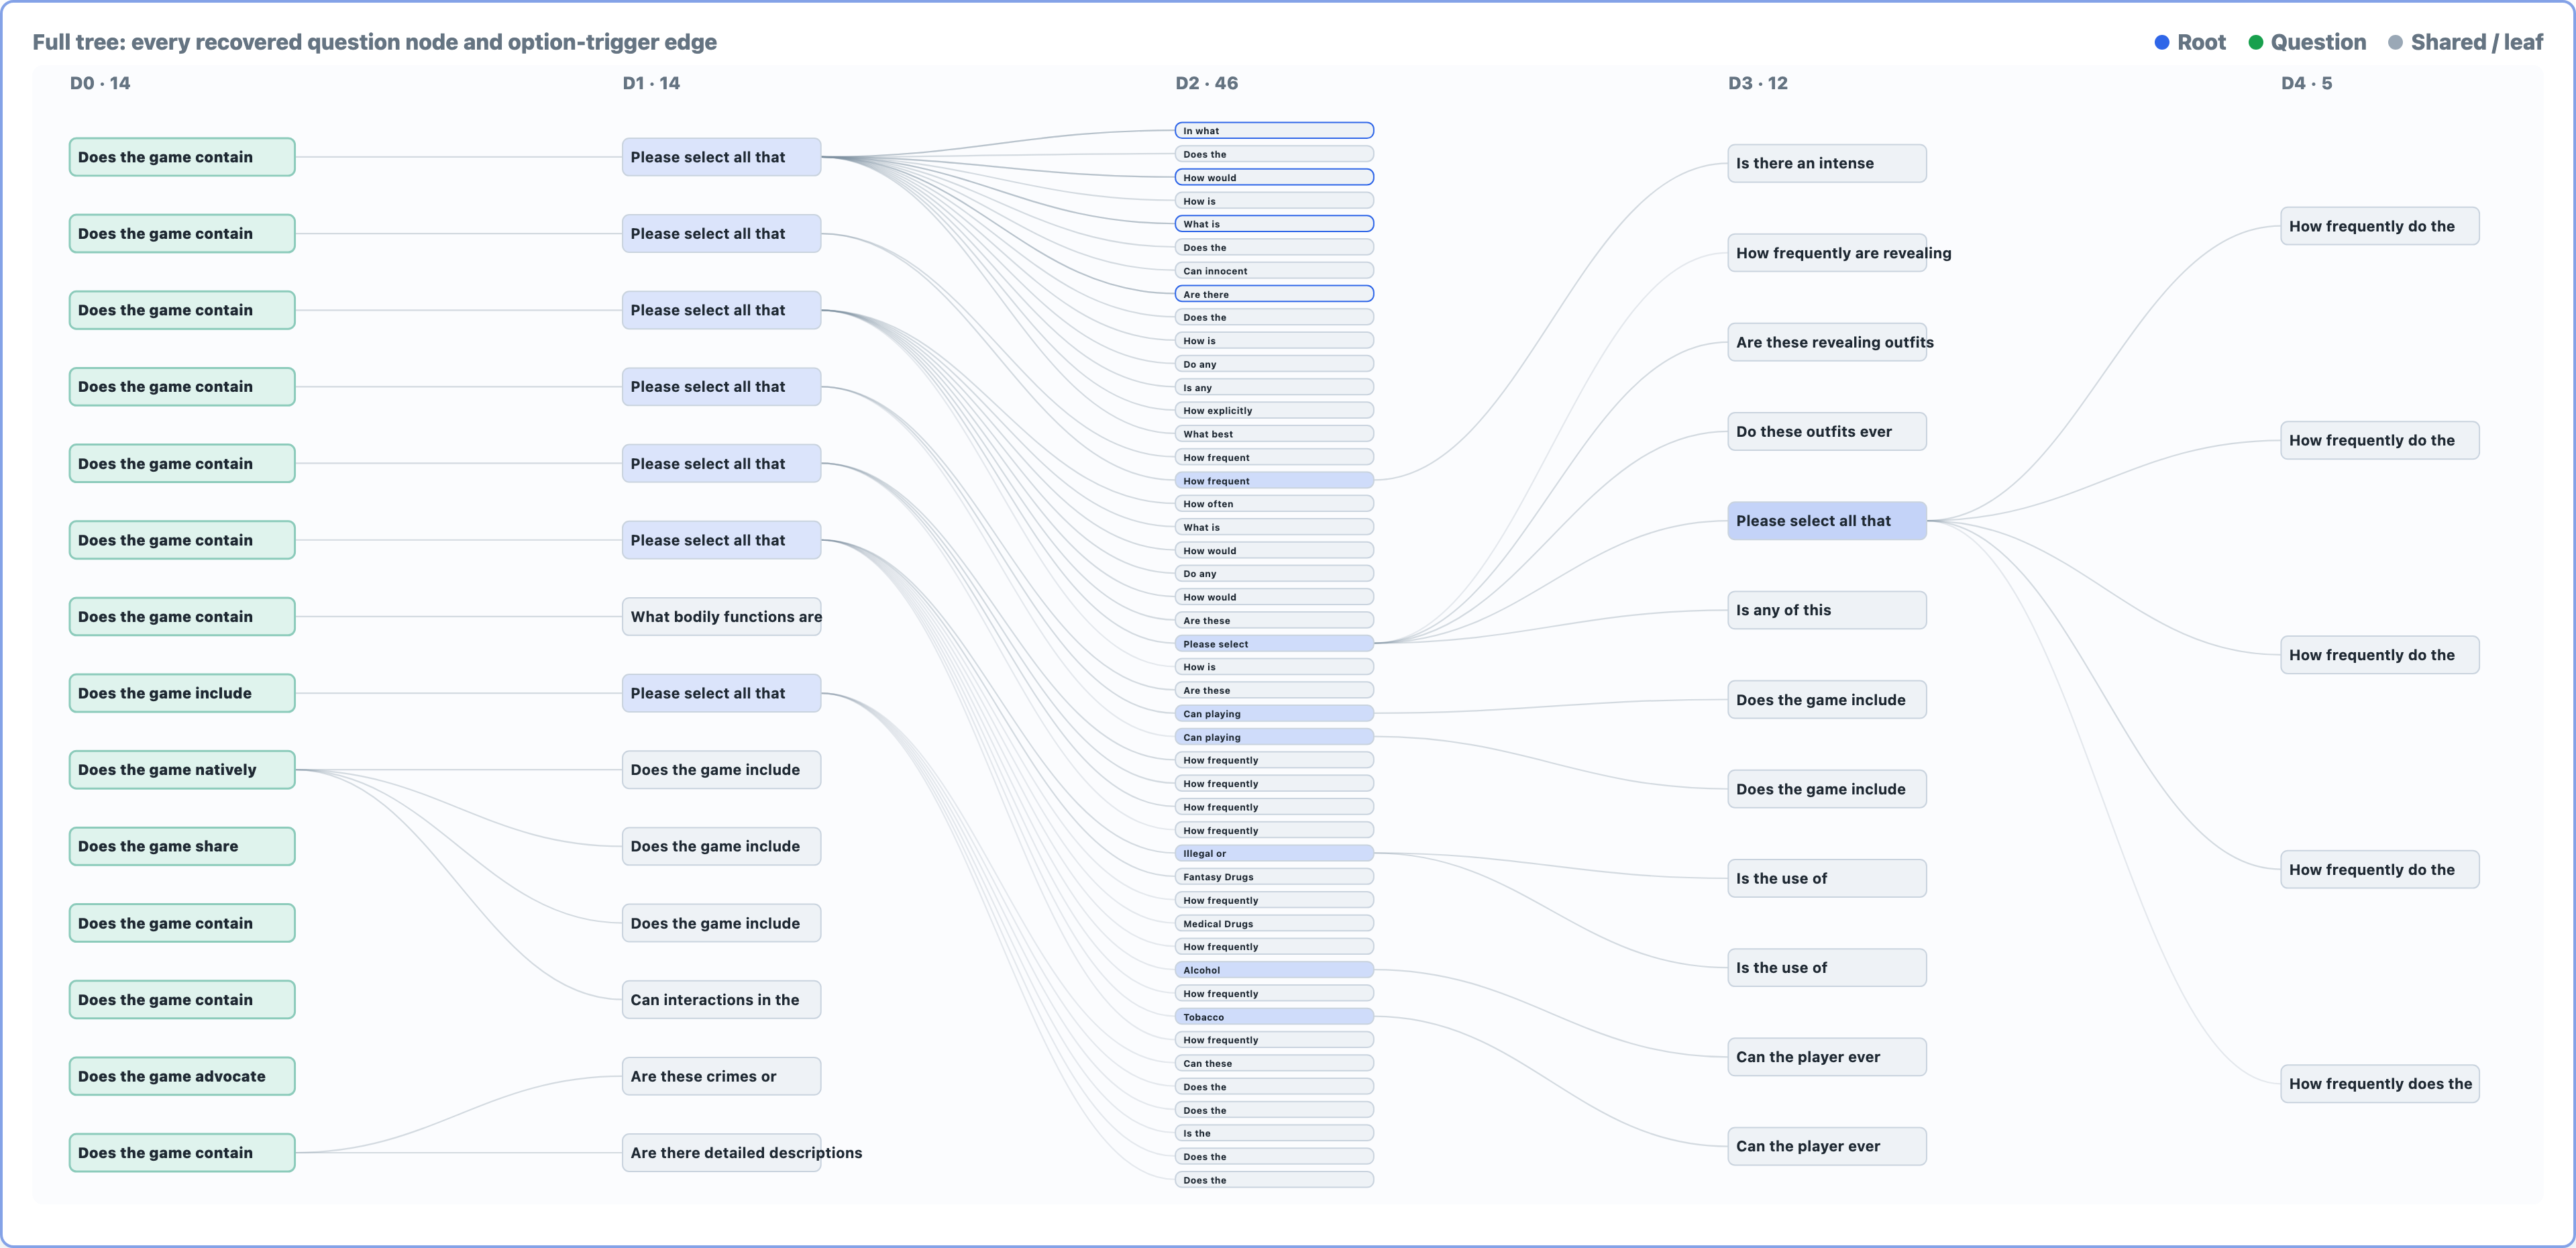
\includegraphics[width=\textwidth]{figures/game_question_graph_tree_only.png}
  \caption{Game Category Questionnaire Topology}
  \label{fig:game-structure}
\end{subfigure}
\hfill
\begin{subfigure}{0.48\textwidth}
  \centering
  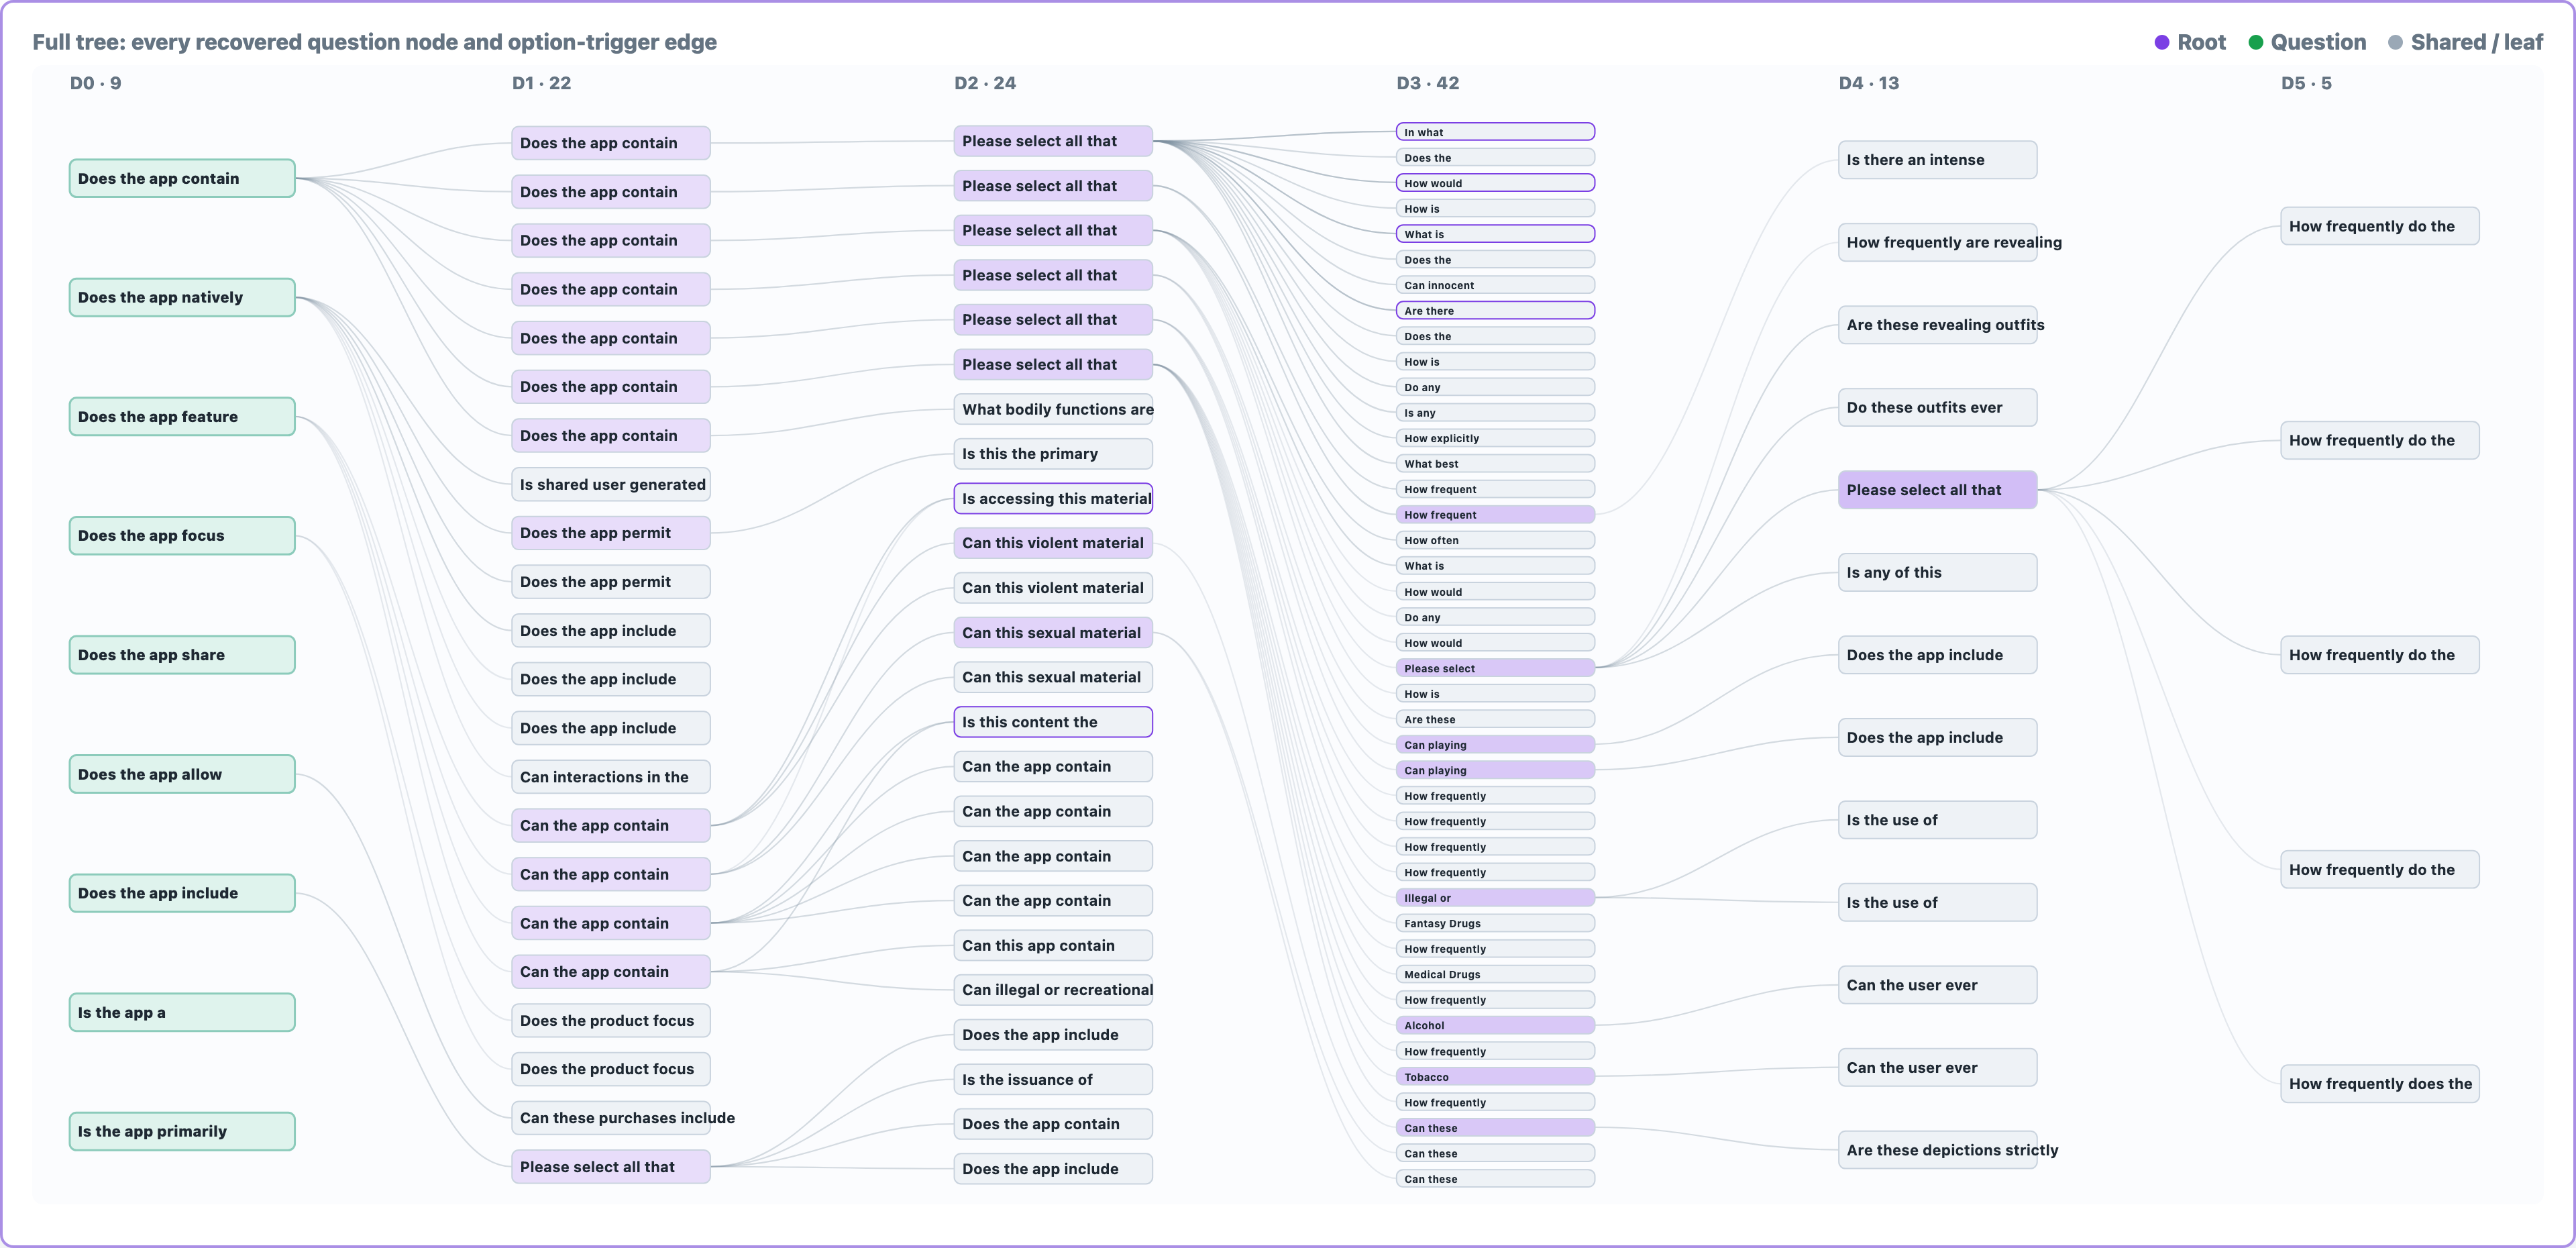
\includegraphics[width=\textwidth]{figures/all_other_question_graph_tree_only.png}
  \caption{All Other App Types Topology}
  \label{fig:other-structure}
\end{subfigure}
\caption{Inspected question structures for two typical categories.}
\label{fig:questionnaire-structures}
\end{figure}

\begin{figure}[H]
\centering
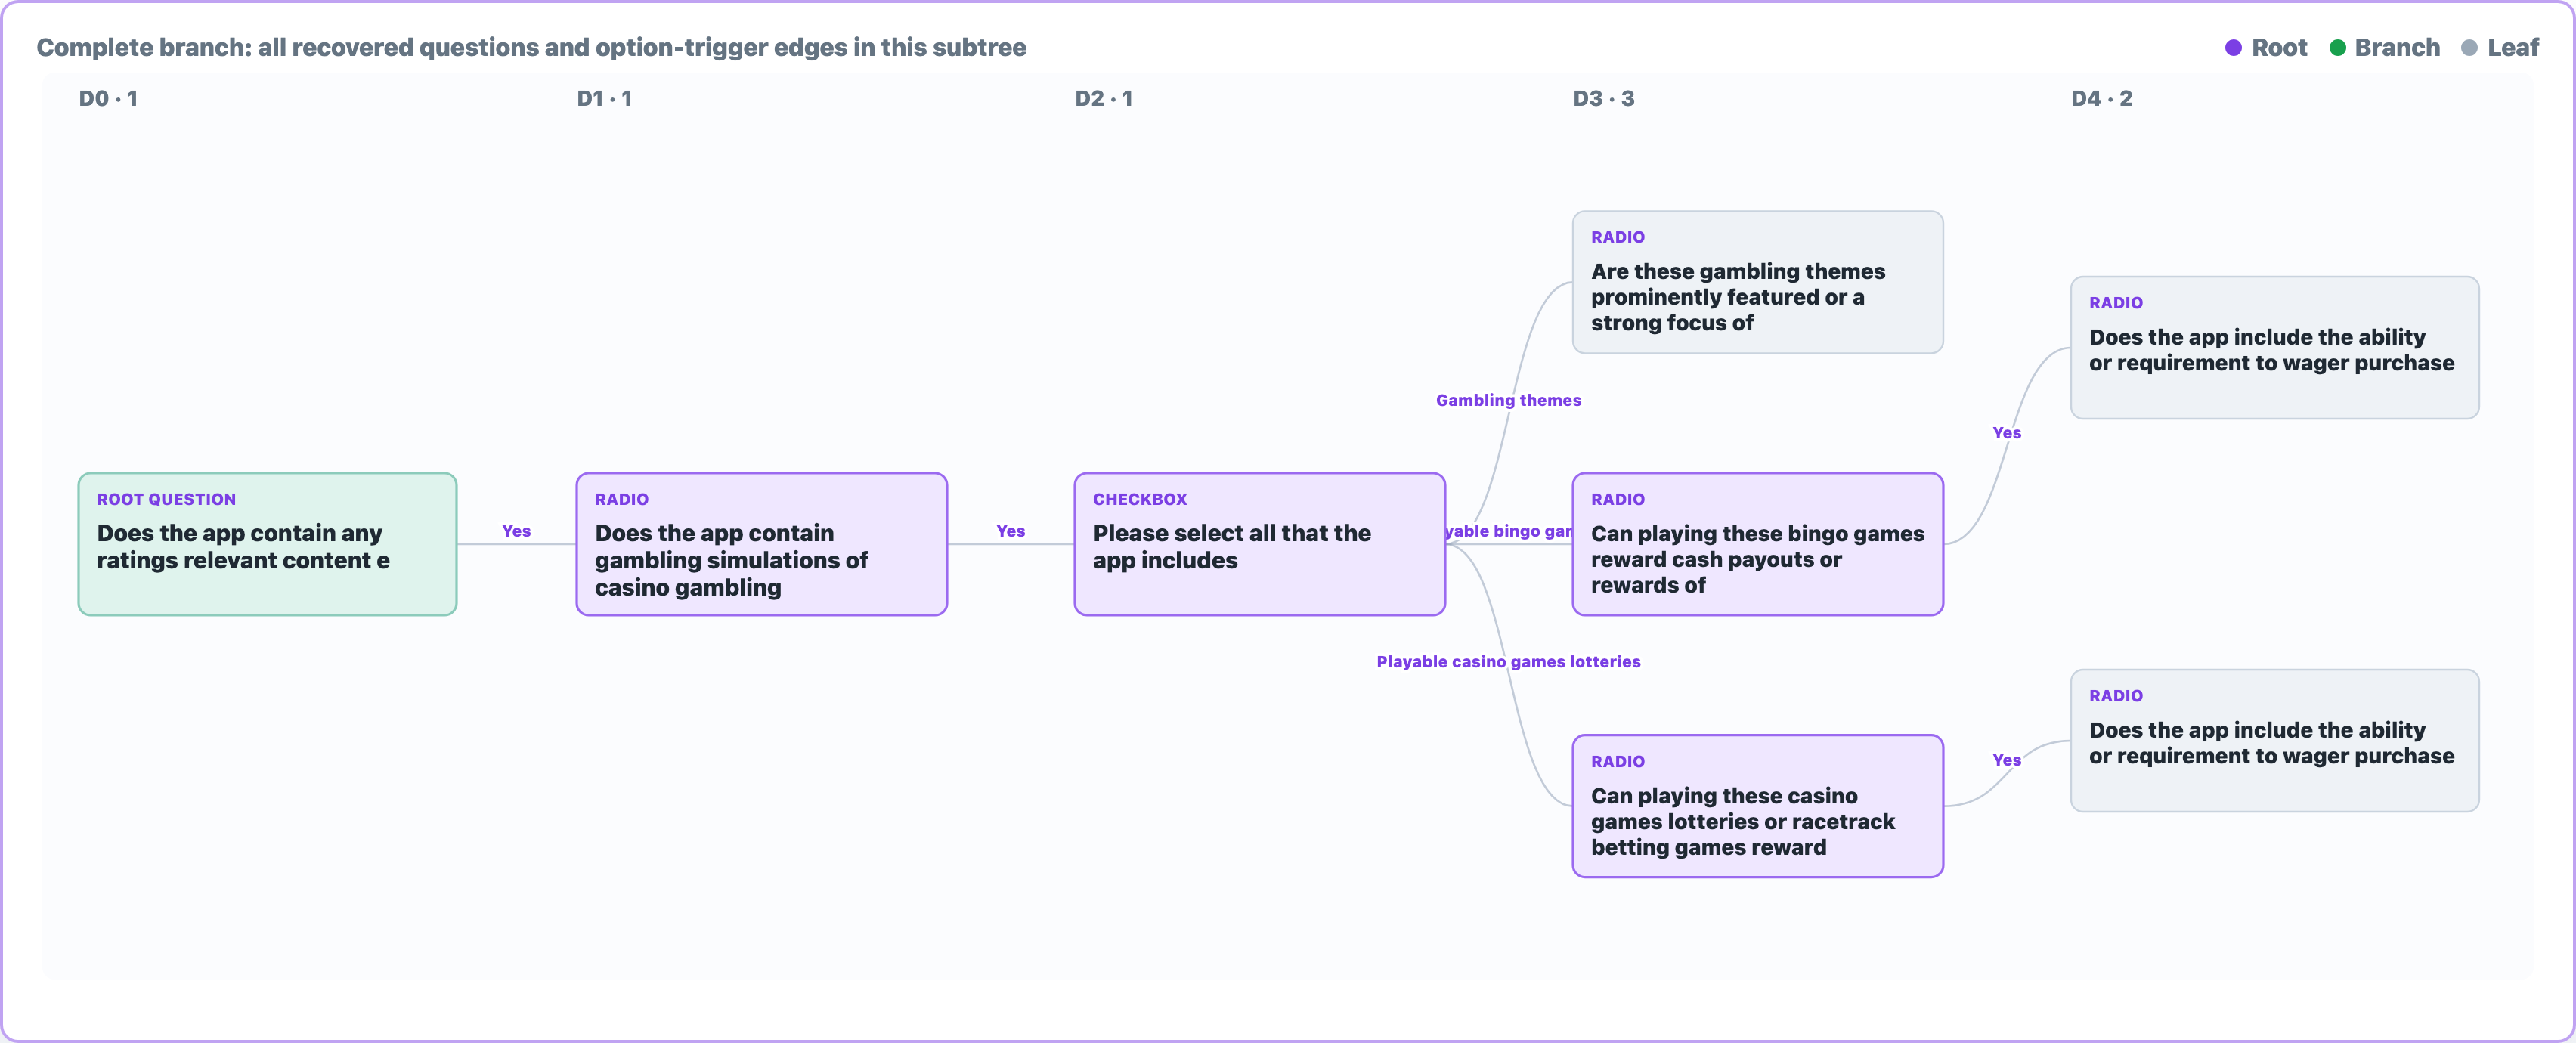
\includegraphics[width=0.72\textwidth]{figures/depth4_branch_example_content.png}
\caption{Example of localized sub-question dependencies (at depth 4).}
\label{fig:question-example}
\end{figure}

The project covers three application categories:
\begin{itemize}[leftmargin=2em]
  \item All Other App Types;
  \item Game;
  \item Social or Communication.
\end{itemize}

Each category triggers a distinct question subtree. For instance, the Game category is more likely to ask about virtual item purchases, simulated gambling, and in-game awards, whereas the Social or Communication category focuses on user-generated content, location sharing, and communication features. The All Other App Types category serves as the general baseline.

\subsection{Sampling Strategy}

Exhaustively combining all options results in an exponential sample space, with many combinations yielding redundant or low-information paths. To compile a diverse and informative training set, we design a multi-tiered sampling strategy:
\begin{enumerate}[leftmargin=2em]
  \item \textbf{Baseline Samples}: Generates low-risk default paths for each category to establish a baseline.
  \item \textbf{Structural Samples}: Systematically varies options along the questionnaire branches to cover all parent-child pathways.
  \item \textbf{Risk-Driven Samples}: Generates dense samples around high-risk elements such as violence, gore, sexual content, drugs, and cash payouts.
  \item \textbf{Borderline Samples}: Targets transitional categories (Everyone 10+, Teen, Mature 17+) to resolve decision boundaries.
  \item \textbf{Coverage-Driven Samples}: Identifies infrequently selected options and prioritizes generating combinations to cover them.
  \item \textbf{Gap-Filling Samples}: Dynamically computes missing or low-frequency reachable paths and injects target samples to fill gaps.
\end{enumerate}

This strategy is highly suited to tree-structured questionnaires compared to random sampling: it avoids massive duplicates of low-risk samples and actively targets high-risk branches and boundary states.

\section{Automated Data Collection}

\subsection{Automated Workflow}

The collection script submits questionnaires automatically in the Google Play Developer Console. The core steps are:
\begin{enumerate}[leftmargin=2em]
  \item Connects to a Chrome instance with an active login session;
  \item Navigates to or restores the content rating questionnaire page;
  \item Selects the target application category and accepts terms;
  \item Answers all visible questions based on the generated sample;
  \item Handles asynchronous rendering, loading spinners, and modal overlays;
  \item Saves the draft and proceeds to the rating Summary page;
  \item Parses the generated age ratings, content descriptors, and interactive elements;
  \item Records the final results, execution evidence, errors, and run parameters;
  \item References checkpoints to continue the batch or retry failed submissions.
\end{enumerate}

\subsection{Core Automation Code}

The code block below demonstrates how the script connects to Chrome via CDP and reuses the open tab. This prevents Google login blocks and slot mismatches.

\begin{lstlisting}[caption={CDP connection and page reuse logic}]
async function openBrowserPage() {
  const browser = await chromium.connectOverCDP(config.cdpUrl);
  const context = browser.contexts()[0] || await browser.newContext();
  const existing = context.pages().find((candidate) =>
    candidate.url().includes('/content-rating')
  );
  const page = existing || context.pages()[0] || await context.newPage();
  return {
    page,
    close: async () => {
      if (typeof browser.disconnect === 'function') browser.disconnect();
    },
  };
}
\end{lstlisting}

The automation script also features robust state recovery. If a page gets stuck in a loading state, throws an error, or displays an overlay, the script detects the current UI state and recovers (e.g., by reloading, backtracking, or restarting the draft) to maintain autonomous collection.

\subsection{Data Quality and Collection Failures}

The final cleaned dataset contains 1,265 valid samples. During collection, 770 failures, 30 validation quarantine events, and 13 rating conflicts were recorded. These events are saved in \code{failures.jsonl}, \code{validation_quarantine.jsonl}, and \code{rating_conflicts.jsonl} to support debugging and sampling adjustments.

\begin{table}[H]
\centering
\caption{Data Quality and Collection Statistics}
\label{tab:quality}
\renewcommand{\arraystretch}{1.25}
\begin{tabular}{lr}
\toprule
Metric & Count \\
\midrule
Cleaned Valid Samples & 1,265 \\
Excluded Samples in Task 3 & 0 \\
Training Samples & 1,012 \\
Testing Samples & 253 \\
Standardized Question Answer Columns & 164 \\
Category-Question Unique Combinations & 218 \\
Territorial Rating Label Columns & 10 \\
Upstream Quarantined Samples & 30 \\
Upstream Rating Conflict Samples & 13 \\
Upstream Execution Failure Events & 770 \\
\bottomrule
\end{tabular}
\end{table}

\section{Data Cleaning and Dataset Analysis}

\subsection{Cleaning Principles}

The goal of data cleaning is to construct a clean tabular format for modeling while strictly preventing label leakage. The cleaning pipeline consists of:
\begin{itemize}[leftmargin=2em]
  \item Verifying schema versions and essential columns;
  \item Validating radio button value compliance;
  \item Corroborating explicit answers against the full questionnaire state;
  \item Verifying path reachability using the question graph to filter out impossible states;
  \item Confirming that territorial ratings match the category's expected output;
  \item Deduplicating sample IDs and identical answer combinations;
  \item Filtering out questionnaire states that produced conflicting ratings across runs;
  \item Encoding structural missing states into unique non-null sentinels.
\end{itemize}

No statistical imputation is performed. "Missing" values in this task represent structural properties of the questionnaire rather than random data loss. For instance, \code{__INACTIVE__} denotes a question that was not triggered by parent answers; \code{__NOT_APPLICABLE__} denotes a question/rating that is irrelevant to the category; and \code{__NONE__} indicates that a visible checkbox question was left unchecked. These states contain key predictive signals.

\subsection{Train/Test Split}

The dataset is partitioned using a deterministic 80/20 holdout split stratified by application category and North American ESRB rating. The seed is fixed to \code{osn-lab2-task3-v1}. This setup:
\begin{enumerate}[leftmargin=2em]
  \item Ensures that the rating label distribution remains identical across the train and test sets;
  \item Guarantees exact reproducibility across different execution environments.
\end{enumerate}

\begin{table}[H]
\centering
\caption{Dataset Category Distribution}
\label{tab:category-distribution}
\renewcommand{\arraystretch}{1.25}
\begin{tabular}{lrrrr}
\toprule
Application Category & Total & Train Set & Test Set & Test Ratio \\
\midrule
All Other App Types & 616 & 492 & 124 & 20.13\% \\
Game & 633 & 507 & 126 & 19.91\% \\
Social or Communication & 16 & 13 & 3 & 18.75\% \\
\midrule
Total & 1,265 & 1,012 & 253 & 20.00\% \\
\bottomrule
\end{tabular}
\end{table}

\begin{table}[H]
\centering
\caption{North American ESRB Rating Distribution}
\label{tab:rating-distribution}
\renewcommand{\arraystretch}{1.25}
\begin{tabular}{lrrrr}
\toprule
Age Rating & Total & Train Set & Test Set & Test Ratio \\
\midrule
Everyone & 182 & 146 & 36 & 19.78\% \\
Everyone 10+ & 138 & 110 & 28 & 20.29\% \\
Teen & 339 & 271 & 68 & 20.06\% \\
Mature 17+ & 365 & 292 & 73 & 20.00\% \\
Adults only 18+ & 241 & 193 & 48 & 19.92\% \\
\midrule
Total & 1,265 & 1,012 & 253 & 20.00\% \\
\bottomrule
\end{tabular}
\end{table}

\subsection{Data Distribution Visualization}

Figure~\ref{fig:data-bars} shows the sample sizes across the age ratings. Everyone 10+ is the minority class, whereas Mature 17+ and Teen are the majority classes. This class imbalance affects the model's recall and F1-scores on intermediate ratings.

\begin{figure}[H]
\centering
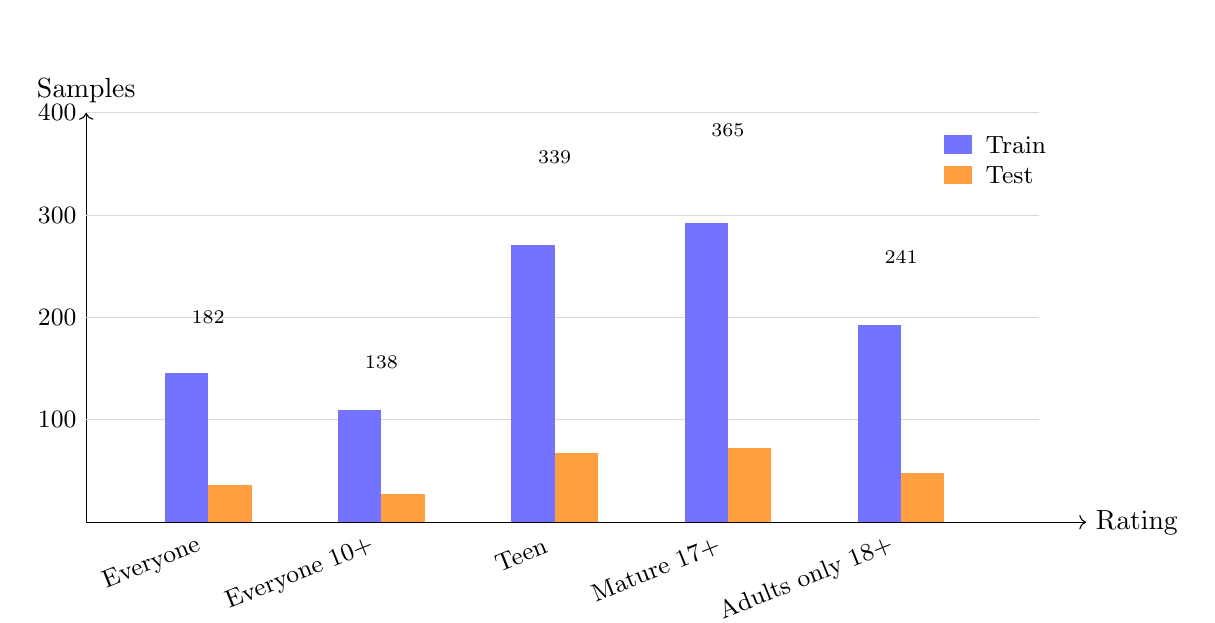
\begin{tikzpicture}[x=1cm,y=0.013cm]
  \draw[->] (0,0) -- (12.7,0) node[right]{Rating};
  \draw[->] (0,0) -- (0,400) node[above]{Samples};
  \foreach \y in {100,200,300,400} {
    \draw[black!15] (0,\y) -- (12.1,\y);
    \node[left] at (0,\y) {\small \y};
  }
  \def\barw{0.55}
  \foreach \x/\name/\train/\test/\total in {
    1/Everyone/146/36/182,
    3.2/Everyone 10+/110/28/138,
    5.4/Teen/271/68/339,
    7.6/Mature 17+/292/73/365,
    9.8/Adults only 18+/193/48/241
  }{
    \fill[blue!55] (\x,0) rectangle ++(\barw,\train);
    \fill[orange!75] (\x+\barw,0) rectangle ++(\barw,\test);
    \node[rotate=22, anchor=east, font=\small] at (\x+0.55,-18) {\name};
    \node[font=\scriptsize] at (\x+0.55,\total+18) {\total};
  }
  \fill[blue!55] (10.9,360) rectangle ++(0.35,18);
  \node[right, font=\small] at (11.3,369) {Train};
  \fill[orange!75] (10.9,330) rectangle ++(0.35,18);
  \node[right, font=\small] at (11.3,339) {Test};
\end{tikzpicture}
\caption{Sample distribution across ESRB rating classes. The numbers represent the total sample count for each rating.}
\label{fig:data-bars}
\end{figure}

\section{Feature Engineering}

\subsection{Input and Output Definition}

The prediction target is \code{rating__north_america}. The model input consists exclusively of:
\begin{itemize}[leftmargin=2em]
  \item \code{category}: The application category;
  \item \code{answer__*}: The answer values for questionnaire items.
\end{itemize}

To prevent label leakage, all other territorial rating columns (e.g., European PEGI, German USK, etc.) are strictly excluded. Even when only predicting the North American rating, using other ratings would grant the model unfair information, since those ratings are generated simultaneously by the same black-box system.

\subsection{Encoding Scheme}

The training dataset from Task 3 is split further to create a validation set. The final split for feature engineering is:
\begin{itemize}[leftmargin=2em]
  \item Train Set: 810 samples;
  \item Validation Set: 202 samples;
  \item Test Set: 253 samples (identical to the Task 3 test set).
\end{itemize}

The encoding scheme is structured as follows:
\begin{enumerate}[leftmargin=2em]
  \item \textbf{Category and Radio fields}: Encoded using one-hot encoding.
  \item \textbf{Checkbox fields}: Checkbox lists are split by the separator \code{ || } and encoded using multi-hot encoding.
  \item \textbf{Structural sentinels}: The strings \code{__INACTIVE__}, \code{__NOT_APPLICABLE__}, and \code{__NONE__} are treated as valid categorical categories.
  \item \textbf{Unseen values}: Any new answer values appearing in the validation or test sets that were not observed in the training set are ignored and recorded in \code{unseen_values.json}.
\end{enumerate}

\begin{table}[H]
\centering
\caption{Feature Engineering Scale}
\label{tab:feature-scale}
\renewcommand{\arraystretch}{1.25}
\begin{tabular}{lr}
\toprule
Metric & Count \\
\midrule
Raw Feature Columns & 165 \\
Category / Radio One-Hot Fields & 133 \\
Checkbox Multi-Hot Fields & 32 \\
Encoded Feature Columns (Dimensions) & 758 \\
Train Samples (Task 4) & 810 \\
Validation Samples (Task 4) & 202 \\
Test Samples (Final) & 253 \\
\bottomrule
\end{tabular}
\end{table}

\subsection{Core Feature Engineering Code}

The Python code snippet below demonstrates our sentinel definition and deterministic validation split logic.

\begin{lstlisting}[language=Python, caption={Labels and structural state definitions}]
MISSING_SENTINELS = {"__INACTIVE__", "__NOT_APPLICABLE__", "__NONE__"}
CHECKBOX_SEPARATOR = " || "
DEFAULT_LABEL_ORDER = [
    "Everyone",
    "Everyone 10+",
    "Teen",
    "Mature 17+",
    "Adults only 18+",
]
\end{lstlisting}

\begin{lstlisting}[language=Python, caption={Deterministic validation splitting stratified by category and rating}]
def deterministic_validation_split(train_df, target_column, validation_ratio, seed):
    strata = train_df["category"].astype(str) + " | " + train_df[target_column].astype(str)
    train_indices = []
    val_indices = []

    for _, group in train_df.assign(_stratum=strata).groupby("_stratum", sort=True):
        records = []
        for idx, row in group.iterrows():
            key = f"{seed}|{row['sample_id']}|{row['_stratum']}"
            records.append((stable_hash(key), idx))
        records.sort()

        n = len(records)
        if n <= 1:
            n_val = 0
        else:
            n_val = max(1, round(n * validation_ratio))
            n_val = min(n_val, n - 1)

        val_indices.extend(idx for _, idx in records[:n_val])
        train_indices.extend(idx for _, idx in records[n_val:])
\end{lstlisting}

\section{Model Training and Parameter Tuning}

\subsection{Model Selection}

We trained and compared four models spanning linear classification, Bagging ensemble trees, and Boosting ensemble trees:

\begin{table}[H]
\centering
\caption{Selected Models and Underlying Hypotheses}
\label{tab:models}
\renewcommand{\arraystretch}{1.3}
\begin{tabularx}{\textwidth}{p{3.7cm}p{3.0cm}X}
\toprule
Model & Type & Selection Rationale \\
\midrule
Logistic Regression & Linear Multi-Class & One-hot and multi-hot features produce high-dimensional sparse representations where linear models provide strong baselines. L1 regularization can select crucial features. \\
Random Forest & Bagging Trees & Learns non-linear interactions and is invariant to feature scaling; serves as a strong tree baseline. \\
LightGBM & Boosting Trees & Fast training and suitable for tabular data; offers rich control parameters (depth, leaves, child samples) to prevent overfit. \\
XGBoost & Boosting Trees & State-of-the-art tabular model; supports column sampling, early stopping, and L1/L2 regularization on leaves. \\
\bottomrule
\end{tabularx}
\end{table}

\subsection{Logistic Regression and Random Forest}

The training script for these two models is located at \code{task5_2_logistic_regression\&random_forest/train_models.py}. We applied balanced class weights to address the rating imbalance. The final hyperparameters are:

\begin{lstlisting}[language=Python, caption={Logistic Regression and Random Forest definitions}]
models = {
    "logistic_regression": LogisticRegression(
        C=10.0,
        l1_ratio=1.0,
        tol=1e-4,
        solver="saga",
        max_iter=5000,
        class_weight=class_weight_by_id,
        random_state=42,
    ),
    "random_forest": RandomForestClassifier(
        n_estimators=500,
        max_depth=None,
        min_samples_leaf=1,
        max_features=0.3,
        min_samples_split=2,
        class_weight=class_weight_by_id,
        random_state=42,
        n_jobs=-1,
    ),
}
\end{lstlisting}

Logistic Regression uses L1 regularization (SAGA solver), enforcing sparsity across the multi-class coefficient weights. Since the feature space is sparse, L1 regularization nullifies irrelevant question choices, isolating the select few that determine rating transitions.

Random Forest's default parameter \code{max_features='sqrt'} performs poorly here, as it only samples ~27 features per split, which frequently misses key question triggers in a 758-dimensional space. By tuning \code{max_features} to 0.3 (allowing each split to evaluate ~228 features), test set Accuracy improved from 0.617 to 0.783, and Macro F1 rose from 0.624 to 0.797.

\subsection{LightGBM and XGBoost}

LightGBM and XGBoost training and tuning are documented in \code{task5_1_lightgbm\&xgboost/ana1.ipynb}. We applied regularized search to prevent overfitting:

\begin{table}[H]
\centering
\caption{LightGBM and XGBoost Hyperparameters}
\label{tab:gbdt-params}
\renewcommand{\arraystretch}{1.25}
\begin{tabular}{lll}
\toprule
Model & Parameter & Optimized Value / Description \\
\midrule
LightGBM & \code{max_depth} & 6 (constrains tree depth) \\
LightGBM & \code{num_leaves} & 15 (restricts leaf size) \\
LightGBM & \code{min_child_samples} & 15 (requires minimum samples per leaf) \\
LightGBM & \code{learning_rate} & 0.1 \\
\midrule
XGBoost & \code{max_depth} & 6 (limits individual tree complexity) \\
XGBoost & \code{subsample} & 1.0 \\
XGBoost & \code{colsample_bytree} & 0.8 (samples 80\% of features per tree) \\
XGBoost & \code{learning_rate} & 0.1 \\
\bottomrule
\end{tabular}
\end{table}

\section{Experimental Results and Model Comparison}

\subsection{Overall Performance}

Table~\ref{tab:model-performance} compares the four models on the test set. Logistic Regression significantly outperforms the tree-based models. XGBoost ranks second, Random Forest third, and LightGBM fourth.

\begin{table}[H]
\centering
\caption{Model Performance Comparison on the Test Set}
\label{tab:model-performance}
\renewcommand{\arraystretch}{1.25}
\begin{tabular}{lccc}
\toprule
Model & Test Accuracy & Test Macro F1 & Test Macro AUC \\
\midrule
Logistic Regression & \textbf{0.921} & \textbf{0.918} & \textbf{0.977} \\
XGBoost & 0.814 & 0.810 & 0.962 \\
Random Forest & 0.783 & 0.797 & 0.945 \\
LightGBM & 0.680 & 0.680 & 0.924 \\
\bottomrule
\end{tabular}
\end{table}

\begin{figure}[H]
\centering
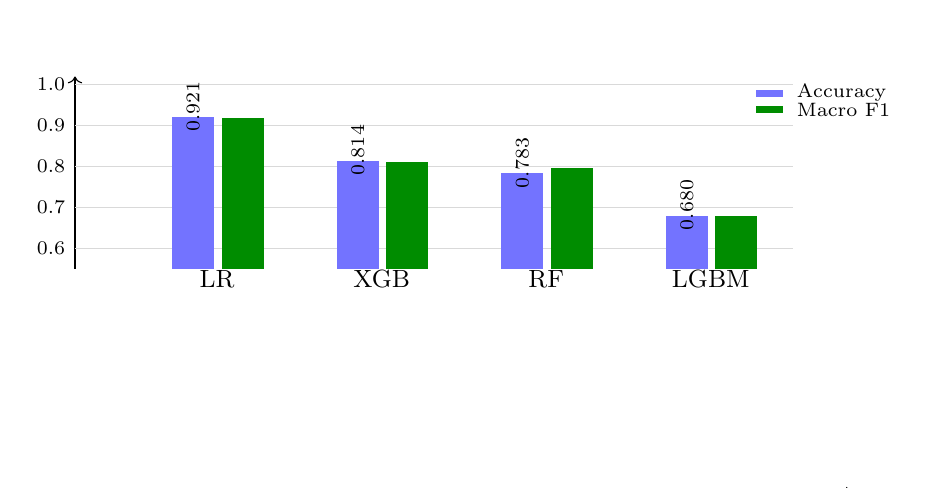
\begin{tikzpicture}[x=1.9cm,y=5.2cm]
  \draw[->] (0,0) -- (5.2,0);
  \draw[->] (0,0.55) -- (0,1.02);
  \foreach \y/\lab in {0.6/0.6,0.7/0.7,0.8/0.8,0.9/0.9,1.0/1.0} {
    \draw[black!15] (0,\y) -- (4.8,\y);
    \node[left,font=\scriptsize] at (0,\y) {\lab};
  }
  \foreach \x/\name/\acc/\f in {
    0.65/LR/0.921/0.918,
    1.75/XGB/0.814/0.810,
    2.85/RF/0.783/0.797,
    3.95/LGBM/0.680/0.680
  }{
    \fill[blue!55] (\x,0.55) rectangle ++(0.28,\acc-0.55);
    \fill[green!55!black] (\x+0.33,0.55) rectangle ++(0.28,\f-0.55);
    \node[font=\small] at (\x+0.30,0.525) {\name};
    \node[font=\scriptsize, rotate=90] at (\x+0.14,\acc+0.026) {\acc};
  }
  \fill[blue!55] (4.55,0.97) rectangle ++(0.18,0.018);
  \node[right,font=\scriptsize] at (4.76,0.979) {Accuracy};
  \fill[green!55!black] (4.55,0.93) rectangle ++(0.18,0.018);
  \node[right,font=\scriptsize] at (4.76,0.939) {Macro F1};
\end{tikzpicture}
\caption{Comparison of Accuracy and Macro F1 across the four models.}
\label{fig:model-bars}
\end{figure}

\subsection{Generalization Gap}

Table~\ref{tab:val-test} compares validation and test set performance for Logistic Regression and Random Forest. Both models display minor generalization gaps, indicating no severe overfitting.

\begin{table}[H]
\centering
\caption{Validation and Test Performance Comparison}
\label{tab:val-test}
\renewcommand{\arraystretch}{1.25}
\begin{tabular}{lcccc}
\toprule
Model & Val Accuracy & Val Macro F1 & Test Accuracy & Test Macro F1 \\
\midrule
Logistic Regression & 0.936 & 0.928 & 0.921 & 0.918 \\
Random Forest & 0.812 & 0.811 & 0.783 & 0.797 \\
\bottomrule
\end{tabular}
\end{table}

\subsection{Classification Report of the Best Model}

Table~\ref{tab:lr-report} displays the class-level performance of our best model, Logistic Regression. Predictions are robust for Everyone, Mature 17+, and Adults only 18+. The Everyone 10+ category has the lowest F1-score due to its small sample size and transitional semantics between Everyone and Teen.

\begin{table}[H]
\centering
\caption{Logistic Regression Test Set Classification Report}
\label{tab:lr-report}
\renewcommand{\arraystretch}{1.25}
\begin{tabular}{lrrrr}
\toprule
Class & Precision & Recall & F1-score & Support \\
\midrule
Everyone & 0.921 & 0.972 & 0.946 & 36 \\
Everyone 10+ & 0.889 & 0.857 & 0.873 & 28 \\
Teen & 0.855 & 0.956 & 0.903 & 68 \\
Mature 17+ & 0.957 & 0.918 & 0.937 & 73 \\
Adults only 18+ & 1.000 & 0.875 & 0.933 & 48 \\
\midrule
Macro Avg & 0.924 & 0.916 & 0.918 & 253 \\
Weighted Avg & 0.925 & 0.921 & 0.921 & 253 \\
\bottomrule
\end{tabular}
\end{table}

\subsection{Confusion Matrix Analysis}

The confusion matrix for Logistic Regression on the test set is shown in Figure~\ref{fig:lr-cm}. Errors are confined to adjacent or semantically overlapping categories:
\begin{itemize}[leftmargin=2em]
  \item 4 Everyone 10+ samples are predicted as Teen;
  \item A few Teen samples are misclassified as Everyone, Everyone 10+, or Mature 17+;
  \item 4 Mature 17+ samples are predicted as Teen;
  \item 3 Adults only 18+ samples are predicted as Teen, and 2 as Mature 17+.
\end{itemize}
These errors are localized along the age spectrum rather than scattered randomly, indicating the model learns a coherent grading scale.

\begin{figure}[H]
\centering
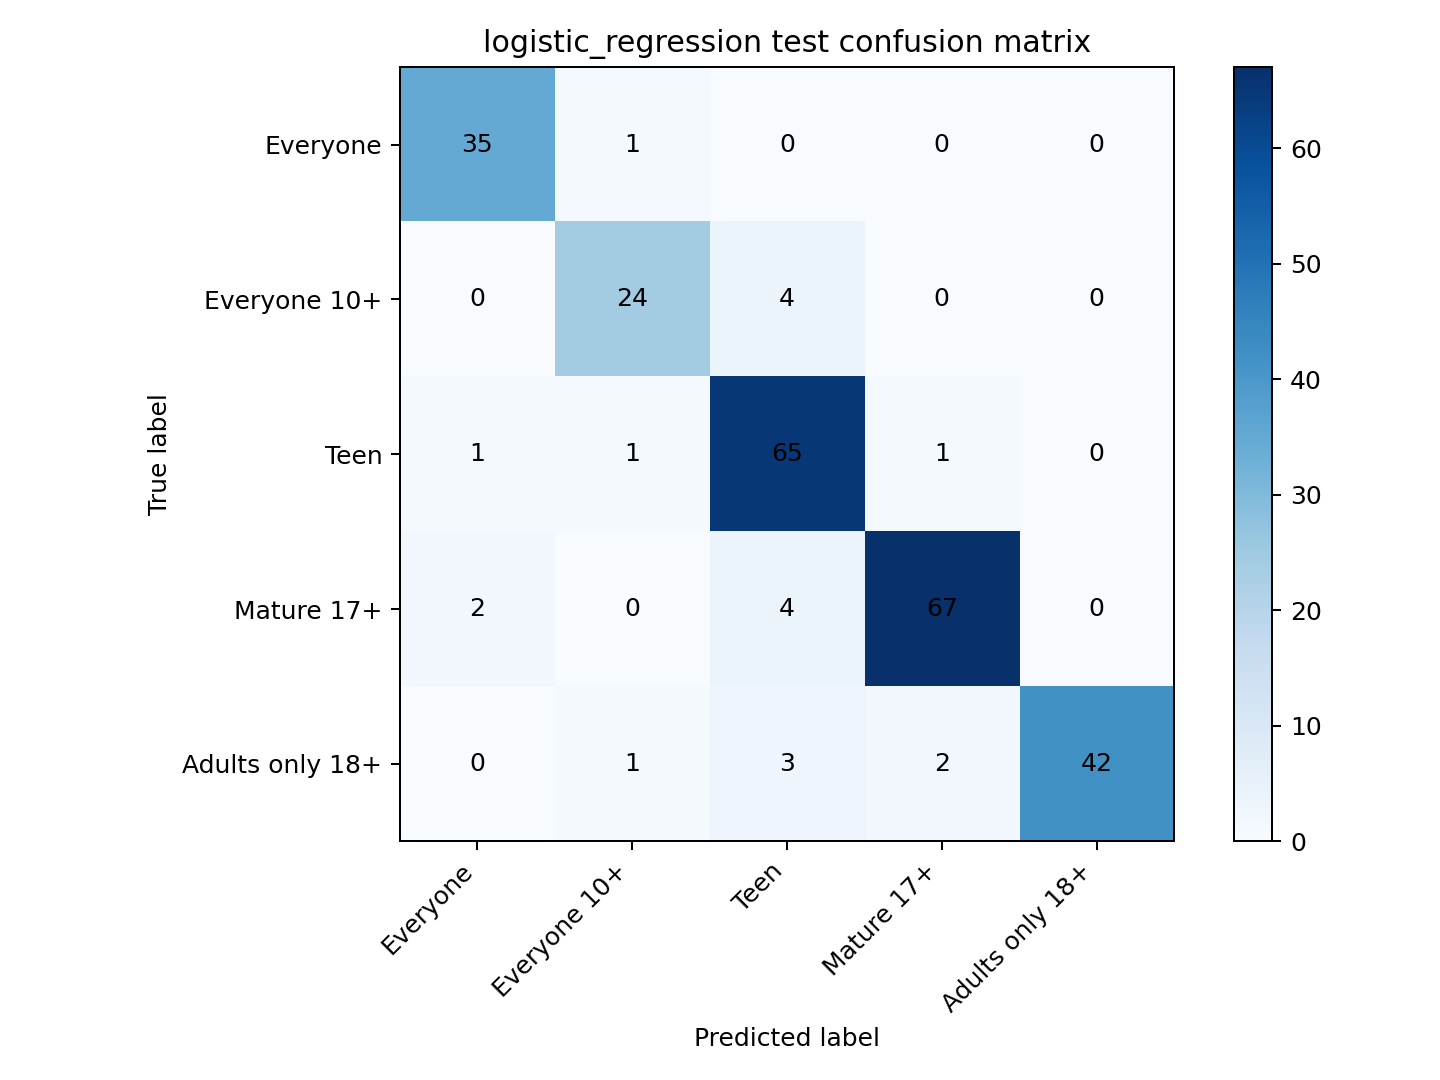
\includegraphics[width=0.72\textwidth]{figures/confusion_matrix_logistic_regression_test.png}
\caption{Logistic Regression test set confusion matrix.}
\label{fig:lr-cm}
\end{figure}

Random Forest's confusion matrix is shown in Figure~\ref{fig:rf-cm}. Compared to Logistic Regression, Random Forest exhibits higher confusion between Teen and Mature 17+, reflecting that tree models require more samples to learn fine-grained boundaries on sparse datasets.

\begin{figure}[H]
\centering
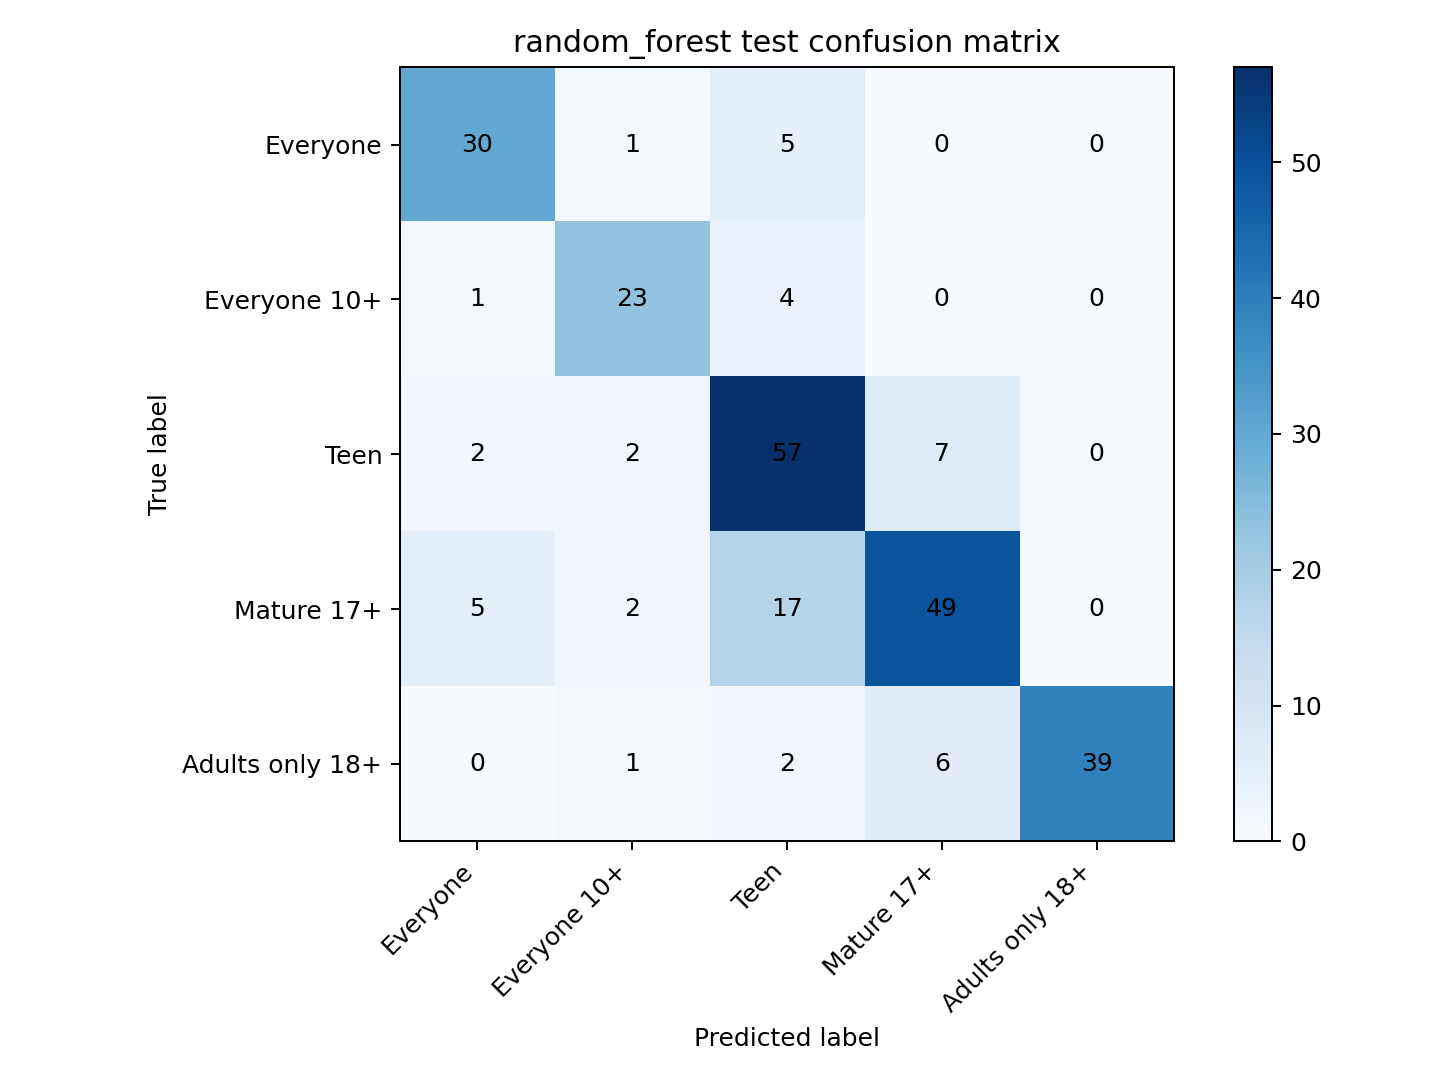
\includegraphics[width=0.72\textwidth]{figures/confusion_matrix_random_forest_test.png}
\caption{Random Forest test set confusion matrix.}
\label{fig:rf-cm}
\end{figure}

The confusion matrices for LightGBM and XGBoost are shown in Figure~\ref{fig:gbdt-cm}. XGBoost outperforms LightGBM but remains inferior to L1-regularized Logistic Regression.

\begin{figure}[H]
\centering
\begin{subfigure}{0.48\textwidth}
  \centering
  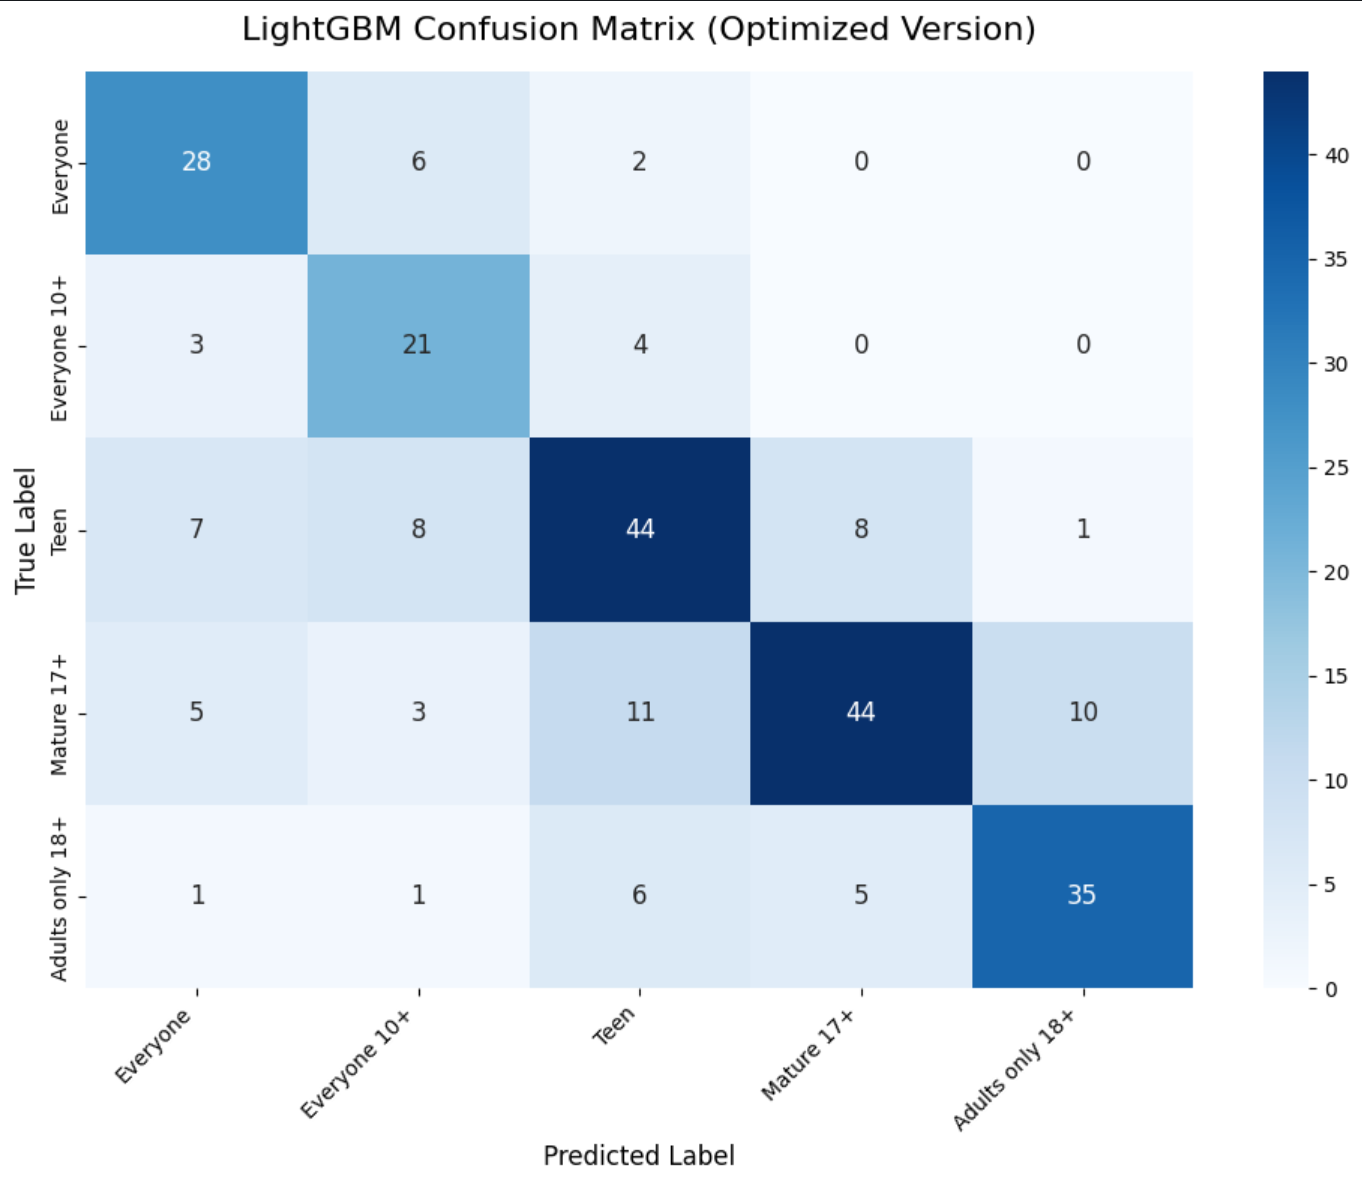
\includegraphics[width=\textwidth]{figures/lightgbm.png}
  \caption{LightGBM}
\end{subfigure}
\hfill
\begin{subfigure}{0.48\textwidth}
  \centering
  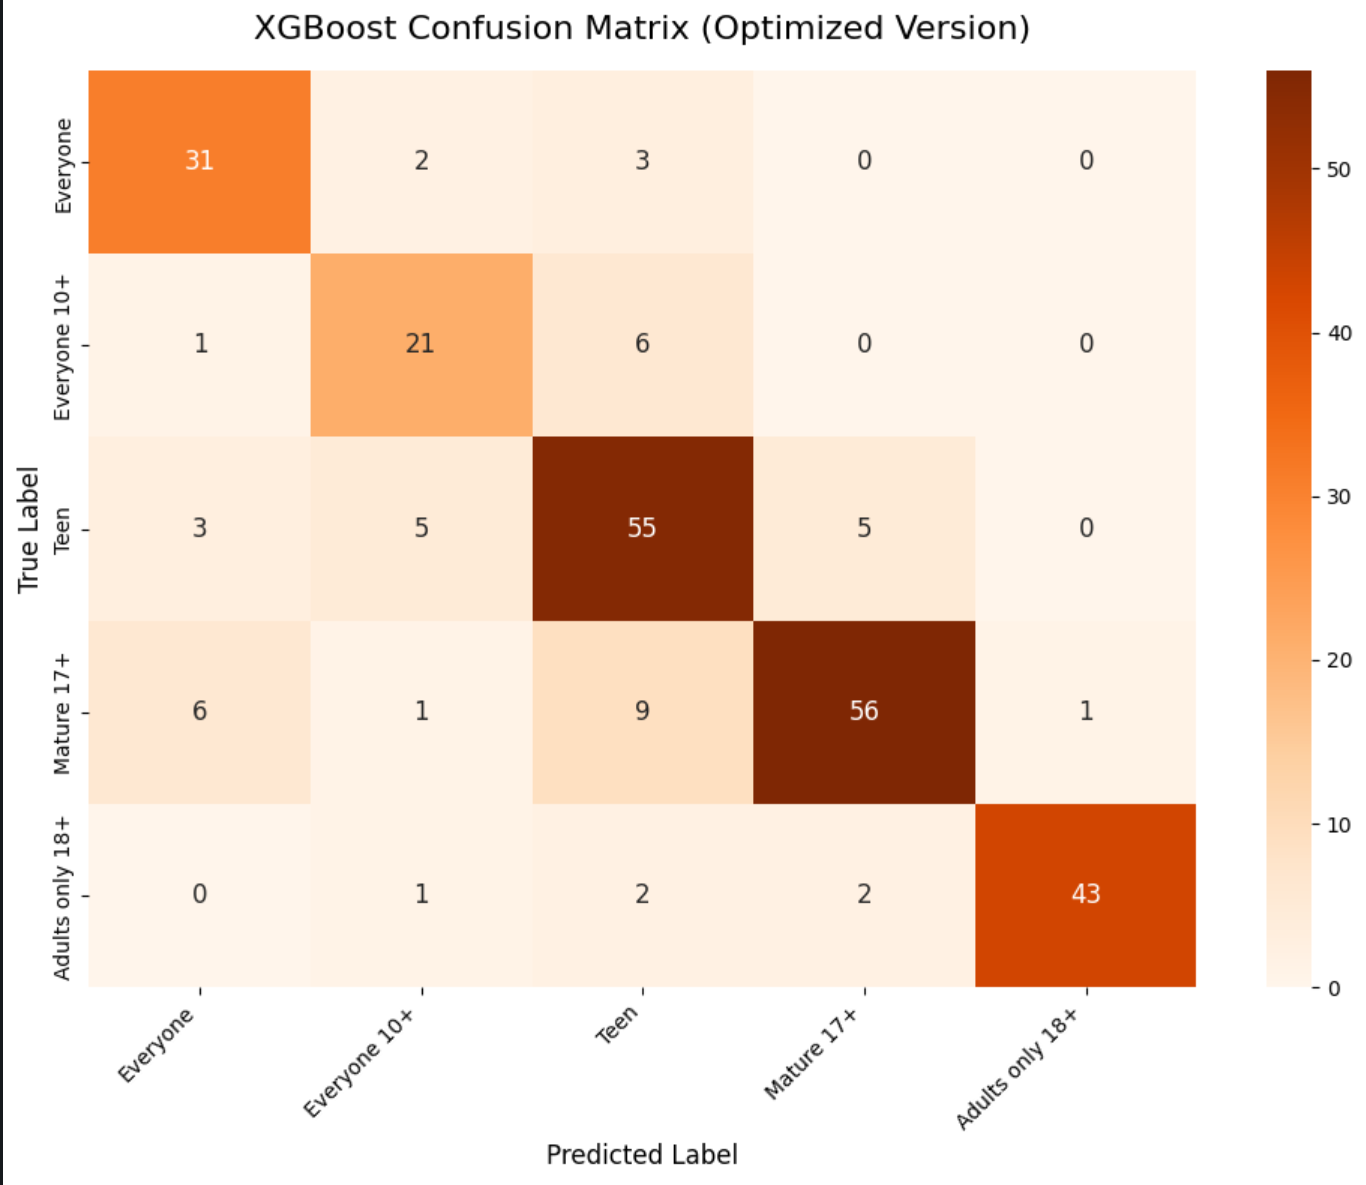
\includegraphics[width=\textwidth]{figures/xgboost.png}
  \caption{XGBoost}
\end{subfigure}
\caption{LightGBM and XGBoost confusion matrices.}
\label{fig:gbdt-cm}
\end{figure}

\section{In-depth Analysis}

\subsection{Why L1 Logistic Regression Performs Best}

The key experimental finding is that L1-regularized Logistic Regression outperforms Random Forest, LightGBM, and XGBoost. This aligns with the properties of the encoded feature representation.

The questionnaire answers are encoded into a 758-dimensional sparse matrix. Each sample activates only a small fraction of features. Google Play's age rating rules likely consist of strong, additive threshold triggers (e.g., presence of gore, frequent sexual themes, drug use, cash gambling). In a one-hot feature space, such triggers translate to linear or piecewise linear boundaries.

The advantages of L1 regularization in this context include:
\begin{enumerate}[leftmargin=2em]
  \item \textbf{Sparsity Alignment}: Zeroes out irrelevant question choices.
  \item \textbf{Mitigating Overfitting}: Given 1,265 samples and 758 features, sparse coefficients reduce the model's capacity, preventing overfitting.
  \item \textbf{High Interpretability}: Non-zero coefficients correspond to concrete questionnaire items, revealing the underlying decision logic.
  \item \textbf{Direct Factor Isolation}: If a single option determines an age jump, a linear classifier directly assigns it a high weight.
\end{enumerate}

Conversely, tree-based models must perform recursive coordinate-aligned splits to replicate additive logic, which demands larger training volumes. LightGBM's leaf-wise growth on small, highly sparse tables easily results underfit or unstable splits.

\subsection{Core Influential Factors}

SHAP values and L1 coefficients highlight the most influential question signals, summarized in Table~\ref{tab:important-features}.

\begin{table}[H]
\centering
\caption{Primary Questionnaire Signals Influencing Age Ratings}
\label{tab:important-features}
\renewcommand{\arraystretch}{1.25}
\begin{tabularx}{\textwidth}{p{1.2cm}p{6.2cm}X}
\toprule
Rank & Signal & Explanation \\
\midrule
1 & Blood/Gore Severity & Higher severity drives ratings towards Teen, Mature 17+, or Adults only 18+. \\
2 & Sexual Themes and Nudity & Major triggers for higher age classes. \\
3 & Erotic/Suggestive Themes Branch & Entry into these sub-questions indicates risk; inactive states conversely signal low risk. \\
4 & Illicit or Recreational Drugs & Increases ratings and defines the Teen vs. Mature 17+ boundary. \\
5 & Gambling, Simulated Gambling & Simulated gambling or cash rewards push ratings significantly higher. \\
6 & User-Generated Interaction & Relevant for Social or Communication categories, though limited by sample size. \\
\bottomrule
\end{tabularx}
\end{table}

These factors correspond directly to established media content rating guidelines: content containing violence, sexuality, drugs, or gambling is restricted to older audiences.

\subsection{Significance of Structural Missingness}

While classical tabular pipelines treat missing values as noise to be imputed, \code{__INACTIVE__}, \code{__NOT_APPLICABLE__}, and \code{__NONE__} represent structural information in this task. Specifically, \code{__INACTIVE__} means a question was bypassed because its parent question received a negative answer (e.g., bypasses drug sub-questions if the app contains no drugs).

Imputing these states would erase this implicit logic. By encoding them as categories, the models directly utilize the bypassed paths. This choice is validated by feature importance rankings, where \code{__INACTIVE__} states regularly appear as strong negative risk indicators.

\subsection{Questionnaire Redundancy and Minimal Feature Sets}

Feature sub-sampling experiments reveal that a small subset of high-weight features is sufficient to replicate the baseline model's performance:

\begin{table}[H]
\centering
\caption{Feature Count vs. Test Accuracy}
\label{tab:feature-redundancy}
\renewcommand{\arraystretch}{1.25}
\begin{tabular}{rrr}
\toprule
Selected Features & Test Accuracy & Relative Performance \\
\midrule
10 & 0.435 & 47\% \\
50 & 0.625 & 68\% \\
200 & 0.933 & 101\% \\
758 & 0.921 & 100\% \\
\bottomrule
\end{tabular}
\end{table}

This demonstrates substantial redundancy in the Google Play questionnaire. Many questions do not affect the North American ESRB rating, or only resolve rare boundary cases. This allows us to:
\begin{enumerate}[leftmargin=2em]
  \item Build compact estimators to predict ratings with minimal question filling;
  \item Understand the high-impact rules to help developers identify critical risk areas.
\end{enumerate}

\subsection{Gray Areas in Rating Boundaries}

Model uncertainty is concentrated on the boundaries of intermediate ratings, such as Teen vs. Mature 17+ and Everyone 10+ vs. Teen. This stems from the subjective nature of these ratings, which depend on fine-grained differences in frequency and presentation. Everyone and Adults only 18+ represent extreme ends of the risk spectrum and are clearly separated. The errors in the confusion matrix are confined to adjacent rating classes, indicating the model learns a smooth risk scale.

\section{Experimental Challenges and Solutions}

\subsection{Data Collection Challenges}

\begin{longtable}{p{4.0cm}p{5.0cm}p{5.5cm}}
\caption{Data Collection Challenges and Solutions}
\label{tab:collection-problems}\\
\toprule
Challenge & Impact & Solution \\
\midrule
\endfirsthead
\toprule
Challenge & Impact & Solution \\
\midrule
\endhead
Google Login Protection & Playwright default headless browser fails login challenges, blocking access to Play Console. & Connected via CDP to a real Chrome profile with an active login session. \\
Account Slot Mismatch & Google URLs map accounts dynamically (e.g., \code{/u/0}, \code{/u/2}). Incorrect accounts lack project permissions. & Reuses open tabs containing `/content-rating` and supports custom URLs via \code{PLAY_CONSOLE_URL}. \\
Unstable Save State & The page can hang on loading spinner after draft saving, missing the rating Summary page. & Implemented state loops, timeout handlers, and recovery rules. \\
Modal Overlays & Pop-up notifications block automated click paths. & Wrote \code{dismissOverlays} to close dialogs and clear the viewport. \\
Dependency Violation & Sampling targets may request hidden questions, causing collection script failure. & Verified reachable path logic via the question graph before execution. \\
Duplicate & Semantic duplication or conflicting rating outputs. & Deduplicated samples at the data stage and exported conflicts to \code{rating_conflicts.jsonl}. \\
\bottomrule
\end{longtable}

\subsection{Modeling Challenges}

\begin{table}[H]
\centering
\caption{Modeling Challenges and Solutions}
\label{tab:model-problems}
\renewcommand{\arraystretch}{1.25}
\begin{tabularx}{\textwidth}{p{4.0cm}X X}
\toprule
Challenge & Impact & Solution \\
\midrule
Class Imbalance & Everyone 10+ has few samples, biasing models towards Teen/Mature 17+. & Applied \code{class_weight='balanced'} or equivalent class multipliers. \\
Target Leakage & Bounding ratings from other regions creates artificial accuracy. & Excluded all rating columns, keeping only \code{category} and \code{answer__*}. \\
High-Dimensional Sparsity & Default tree settings fail to sample informative splits. & Scaled \code{max_features} to 0.3 for Random Forest and restricted tree depth with column sub-sampling for boosting models. \\
LightGBM Underfitting & Yields an F1-score of only ~0.680 on the test set. & Evaluated parameter configurations, referencing the mismatch between tree partitioning and sparse linear logic. \\
Borderline Ambiguity & Confusion on Everyone 10+ / Teen / Mature 17+. & Monitored Macro F1 and analyzed error localization using confusion matrices. \\
\bottomrule
\end{tabularx}
\end{table}

\section{Group Division of Labor}

This project spans web automation, data engineering, feature modeling, and analysis. The group adopted a modular workflow. The role distribution is detailed in Table~\ref{tab:division}.

\begin{table}[H]
\centering
\caption{Group Member Division of Labor}
\label{tab:division}
\renewcommand{\arraystretch}{1.35}
\begin{tabularx}{\textwidth}{p{2.5cm}X}
\toprule
Member & Core Responsibilities \\
\midrule
Yuhan Chen & Project repository maintenance; Google Play Developer Console automation pipeline; questionnaire structure inspection, sample collection, and database maintenance. \\
Jiashun Shi & Raw data processing and pipeline engineering: deduplication, missing value checks, quarantined outlier removal, column name standardization, and train/test splits. \\
Bofan Chen & Feature engineering: raw question mapping, structural sentinel management, one-hot / multi-hot encoding, and feature/label dictionaries. \\
Zihan Chen & LightGBM and XGBoost training and parameter tuning, boosting model evaluation, and comparative performance analysis. \\
Zixuan Wang & Logistic Regression and Random Forest model training, parameter sweeps, model serialization, and metric reporting. \\
\bottomrule
\end{tabularx}
\end{table}

The project steps are highly connected: collection results drive feature updates, and model errors suggest areas requiring further targeted sampling. The group operated as a collaborative closed loop.

\section{Major Project Findings}

Our experimental analysis yields the following conclusions:
\begin{enumerate}[leftmargin=2em]
  \item \textbf{Google Play Age Ratings are Highly Predictable}: Logistic Regression achieved a test Accuracy of 0.921 and a Macro F1 of 0.918, indicating a stable mapping between questionnaire answers and ESRB ratings.
  \item \textbf{Linear Models Fit High-Dimensional Sparse Inputs Best}: L1-regularized Logistic Regression outperformed tree architectures, demonstrating that content rules act as sparse linear triggers in one-hot space.
  \item \textbf{Violence, Sex, Drugs, and Gambling are Key Triggers}: These elements have the highest predictive weight, aligning with established rating standards.
  \item \textbf{Questionnaire Topology Contains Information}: Structural missingness states like \code{__INACTIVE__} are predictive features that represent untriggered sub-branches, and should not be imputed.
  \item \textbf{Substantial Redundancy Exists}: The model matches baseline performance using only ~200 of the 758 features.
  \item \textbf{Transitional Boundaries present High Ambiguity}: Misclassifications are restricted to adjacent categories (Everyone 10+ vs. Teen vs. Mature 17+).
\end{enumerate}

\section{Limitations and Future Directions}

\subsection{Current Limitations}

\begin{enumerate}[leftmargin=2em]
  \item \textbf{Sparse Social/Communication Samples}: Only 16 samples were collected for this category (3 in the test set), preventing reliable modeling.
  \item \textbf{Data Scale}: While satisfying the 1,000-sample limit, 1,265 samples are relatively small for a 758-dimensional space.
  \item \textbf{Temporal Drift}: The rating logic is a black-box system that Google may update, and current rules reflect a snapshot of the console.
  \item \textbf{North American Focus}: We focused on \code{rating__north_america}, leaving regional differences unanalyzed.
  \item \textbf{Correlation vs. Causation}: L1 coefficients show statistical correlation rather than Google's internal causal code.
\end{enumerate}

\subsection{Future Directions}

We propose the following directions:
\begin{itemize}[leftmargin=2em]
  \item Expand sampling for the Social or Communication category;
  \item Use active learning to query samples near rating boundaries;
  \item Model other jurisdictions (PEGI, USK, ACB) and analyze cross-regional rules;
  \item Extract symbolic decision trees from high-weight L1 features;
  \item Calibrate model probabilities to output confidence levels for developers;
  \item Package scripts into a stable execution pipeline independent of interactive browser state.
\end{itemize}

\section{Conclusion}

This project reverse models the Google Play age rating questionnaire. Starting from dynamic questionnaire inspection, we designed a multi-tiered sampling strategy, automated submission and collection using Playwright, and compiled a dataset of 1,265 samples. We trained and compared Logistic Regression, Random Forest, LightGBM, and XGBoost on 758-dimensional features.

L1-regularized Logistic Regression achieved the highest accuracy, with 0.921 Accuracy, 0.918 Macro F1, and 0.977 Macro AUC on the test set. This confirms that the underlying rating system can be modeled with high accuracy using data-driven methods. Violence, drugs, sexuality, and gambling are the main drivers of ratings, and structural missingness represents key information.

Overall, the project successfully completed the data collection, feature engineering, modeling, comparison, and analysis requirements, providing insight into Google Play's age rating mechanism.

\appendix
\section{Experiment Replication Commands}

\begin{lstlisting}[language=bash, caption={Main replication commands}]
# Install Node dependencies
npm install

# Inspect questionnaire structure
CDP_URL="http://127.0.0.1:9222" npm run inspect:questionnaire

# Run sampling
CDP_URL="http://127.0.0.1:9222" npm run run:samples

# Build and validate Dataset V2
npm run build:dataset-v2
npm run validate:dataset-v2

# Feature engineering
python task4_feature_engineering/scripts/build_features.py

# Train Logistic Regression and Random Forest
python "task5_2_logistic_regression&random_forest/train_models.py"
\end{lstlisting}

\section{Key Output Files}

\small
\begin{longtable}{p{6.2cm}p{8.4cm}}
\caption{Key Project Output Files}
\label{tab:outputs}\\
\toprule
File Path & Description \\
\midrule
\endfirsthead
\toprule
File Path & Description \\
\midrule
\endhead
\code{dataset_v2/samples.jsonl} & Primary dataset containing deduplicated samples. \\
\code{dataset_v2/}\\\code{coverage_report.json} & Distribution metrics for categories, ratings, and questions. \\
\code{task3_data_cleaning/}\\\code{output/clean_dataset.csv} & Full cleaned dataset. \\
\code{task3_data_cleaning/}\\\code{output/train.csv} & Task 3 training split. \\
\code{task3_data_cleaning/}\\\code{output/test.csv} & Task 3 test split. \\
\code{task4_feature_engineering/}\\\code{output/X_train.npz} & Sparse feature matrix for training. \\
\code{task4_feature_engineering/}\\\code{output/feature_dictionary.csv} & Feature mapping back to raw questionnaire options. \\
\code{task4_feature_engineering/}\\\code{output/label_mapping.json} & Target rating indices. \\
\code{task5_2_logistic_regression}\\\code{\&random_forest/output/}\\\code{model_comparison.csv} & Metrics for Logistic Regression and Random Forest. \\
\code{task5_2_logistic_regression}\\\code{\&random_forest/output/}\\\code{metrics.json} & Run parameters and validation/test metrics. \\
\code{task5_2_logistic_regression}\\\code{\&random_forest/output/*.png} & Plot files for confusion matrices. \\
\code{task5_1_lightgbm\&xgboost/}\\\code{img/*.png} & Plot files for LightGBM and XGBoost confusion matrices. \\
\bottomrule
\end{longtable}
\normalsize

\section{References}

\begin{enumerate}[leftmargin=2em]
  \item Google Play Developer Console: \url{https://play.google.com/console/developers}
  \item Project Repository: \url{https://github.com/CYH0415/OSN-Lab-Main}
  \item Playwright Documentation: \url{https://playwright.dev/}
  \item scikit-learn Documentation: \url{https://scikit-learn.org/}
  \item XGBoost Documentation: \url{https://xgboost.readthedocs.io/}
  \item LightGBM Documentation: \url{https://lightgbm.readthedocs.io/}
\end{enumerate}

\label{LastPage}
\end{document}
